\documentclass[review,preprint,12pt]{elsarticle}
\usepackage{graphicx}
\usepackage{amssymb,amsmath}
%\usepackage{subfigure}
\usepackage{makeidx}
\usepackage{booktabs,ctable,tabulary,multirow,color}
\usepackage{nomencl}
\usepackage{textcomp}
\usepackage{colortbl}
\usepackage[nice]{nicefrac}
\usepackage{subfig}
\usepackage{graphicx}



\newcommand{\varA}[1]{{\operatorname{#1}}}
\newcommand{\varB}[1]{{\operatorname{\mathit{#1}}}}

\makenomenclature

\RequirePackage{ifthen}
\renewcommand{\nomgroup}[1]{%
\ifthenelse{\equal{#1}{A}}{\item[\textbf{Roman letters}]}{%
\ifthenelse{\equal{#1}{B}}{\item[\textbf{Greek letters}]}{}}{%
\ifthenelse{\equal{#1}{C}}{\item[\textbf{Subscripts}]}{}}{%
\ifthenelse{\equal{#1}{D}}{\item[\textbf{Abbreviations}]}{}}}

\journal{Applied Thermal Engineering}

\begin{document}

\begin{frontmatter}

\title{Development of an Active Magnetic Regenerator Model in Python using the Finite Volume Method}
\author{Gusttav B. Lang}
\author{Jaime A. L. Cadena}
\author{Alan T. D. Nakashima}
\author{Henrique N. Bez}
\author{Jader R. Barbosa Jr.}
\ead{jrb@polo.ufsc.br}
\address{POLO Research Laboratories for Emerging Technologies in Cooling and Thermophysics, Department of Mechanical Engineering, Federal University of Santa Catarina (UFSC), Florian\'{o}polis, SC, 88040900, Brazil, Phone/Fax: (+ 55) 48 3721-7900}

\begin{abstract}

Falar que é open source e a importancia disso

\end{abstract}

\end{frontmatter}

\vspace{0.5cm}

\noindent {\bf Keywords:} Magnetic refrigeration, active magnetic regenerator (AMR), finite volume method (FVM), Python.

\printnomenclature[1.4cm]

\pagebreak

\section{Introduction}

multicamadas com primeira ordem?


\section{Mathematical Model}


As a volume average approach was adopted, the macroscopic momentum equation is given by \cite{Kaviany1995,Nield2006}:

\begin{equation}
\frac{\rho_\textrm{f}}{\varepsilon}\Biggl(\frac{\partial\vec{v}}{\partial t} + \vec{v}\cdot\nabla\vec{v}\Biggr) = -\nabla P + \rho_\textrm{f}\vec{\textrm{f}} + \frac{\mu_\textrm{f}}{\varepsilon}\nabla^2\vec{v} - \frac{\mu_\textrm{f}}{K}\vec{v} -
\frac{c_\textrm{E}\rho_\textrm{f}}{K^{1/2}}|\vec{v}|\vec{v}
\label{BrinkFroch}
\end{equation}

\noindent where the left term is the macroscopic inertial force and the terms on the right represent the pore pressure gradient, body force, macroscopic viscous shear stress (Brinkman viscous term), microscopic shear stress (Darcy term) and microscopic inertial force (Ergun inertial term), respectively. The following simplifying assumptions were also made \cite{Trevizoli2015}:

\begin{enumerate}
\item  One dimensional flow;
\item  Laminar, incompressible fluid flow;
\item  Low porosity medium, i.e., $\varepsilon <$ 0.6;
\item  Absence of body forces.
\end{enumerate}

After the application of the former assumptions in Eq.~\eqref{BrinkFroch}, it is obtained:

\begin{equation}
\frac{\rho_\textrm{f}}{\varepsilon}\Biggl(\frac{\partial u}{\partial t}\Biggr) = -\frac{\partial P}{\partial x} - \frac{\mu_\textrm{f}}{K}u - \frac{c_\textrm{E}\rho_\textrm{f}}{K^{1/2}}|u|u
\label{BrinkFrochSimplified}
\end{equation}

\noindent where $\rho$ is the density, $u$ is the superficial (Darcian) flow velocity, $t$ is the time, $P$ is the pressure, $x$ is the regenerator axial direction, $\mu$ is the dynamic viscosity, $K$ is the permeability of the porous media and $c_{E}$ is the Ergun constant. $K$ and $c_{E}$ depends on the solid geometry and the matrix  porosity. \textcolor{red}{In this thesis, only packed bed of spheres will be evaluated, for which these variables are calculated as \cite{Ergun1952}:}


The macroscopic energy balance for the solid phase is given by \cite{Engelbrecht2004,Trevizoli2015}:

\begin{equation}
\rho_\textrm{s} c_\textrm{H}(T,H)(1-\varepsilon)\frac{\partial T_\textrm{s}}{\partial t} = h(x) \beta (T_\textrm{f}-T_\textrm{s}) + (1-\varepsilon)k^\textrm{eff}_\textrm{s}\frac{\partial^{2} T_\textrm{s}}{\partial x^{2}} + \dot{q}_\textrm{MCE}
\label{SolidEnergyEquation}
\end{equation}

\noindent where the term on is the solid thermal inertia, and the terms on the right are due to interstitial heat convection calculated using a convective heat transfer coefficient, $h$, which is responsible for the thermal couple between the solid and fluid phases, axial heat conduction and the magnetocaloric effect modeled as a source term (if applicable), respectively. $\rho_\textrm{s}$ is the solid density and $k^\textrm{eff}_\textrm{s}$ is the effective thermal conductivity of the solid \cite{Kaviany1995,Nield2006}. $\beta$ (or compactness factor) is the surface area density, defined as the ratio of the interstitial area, which for packed bed spheres it is given by \cite{Kaviany1995}:


\textcolor{red}{citar henrique propriedades dos materiais}
\textcolor{red}{descrever EMC}


As the momentum equation is solved uncoupled, the flow velocity and pressure drop are an input in the fluid energy solver. All of the assumptions made in the momentum equation are also applied for the solid and fluid energy equations, except that $\mu_\textrm{f}$ is not considered constant, since in the range of $\Delta T_\textrm{span}$ used in this thesis $\mu_\textrm{f}$ can vary over five time. The macroscopic energy balance for the fluid phase is given by \cite{Engelbrecht2004,Trevizoli2015}:

\begin{equation}
\rho_\textrm{f} c_\textrm{p,f}(T) \left( \varepsilon \frac{\partial T_\textrm{f}}{\partial t} +  u\frac{\partial T_\textrm{f}}{\partial x} \right) = h(x)\beta(T_\textrm{s}-T_\textrm{f})  + \Biggl|u\frac{\partial P}{\partial x}\Biggr| + \nonumber
\end{equation}
\begin{equation}
\varepsilon\bigl[k^\textrm{eff}_\textrm{f} + \rho_\textrm{f}(T) c_\textrm{p,f}(T)D_{||}\bigr]\frac{\partial^{2} T_\textrm{f}}{\partial x^{2}} +  \dot{q}_\textrm{csg}
\label{FluidEnergyEquation}
\end{equation}

\noindent where the terms on the left are the thermal inertia and axial advection, and the terms on the right are the interstitial heat convection term, the viscous dissipation, the axial conduction and the casing heat transfer terms, respectively \cite{Kaviany1995, Nield2006}. $c_\textrm{p,f}$ is the fluid specific heat capacity, $k^\textrm{eff}_\textrm{f}$ is the the fluid phase effective thermal conductivity and $D_{||}$ is the longitudinal thermal dispersion, proper of porous medium analyses.

The casing heat transfer modeling main goal is to determine the heat transfer rate per unit volume through the regenerator casing wall, $\dot{q}_\textrm{csg}$. This loss is  very important for an AMR model, because there is little room for a good thermal insulation and, as a result, the heat gained from the external environment can deteriorate the AMR performance \cite{Engelbrecht2008,Trevizoli2014,Trevizoli2016b}. Moreover, the inclusion of this model enables the optimization of the casing thickness for specific geometry conditions. $\dot{q}_\textrm{csg}$ was included as a source term in the fluid energy equation Eq.~\eqref{FluidEnergyEquation}. 

The following assumptions are considered in the casing heat transfer modeling \cite{Trevizoli2015}:

\begin{enumerate}
\item  The heat transfer in the wall and air gap is two-dimensional;
\item  The air properties are constant and obtained at an average air temperature;
\item  The wall properties are constant and depend only on the wall material. However, the transversal and longitudinal thermal conductivities can be different (anisotropic characteristic). Thus, for the G10 casing $k_\textrm{wall,y} \neq k_\textrm{wall,x}$.
\item  Since the thermal mass of the magnetic circuit is very large, the temperature of the magnet is assumed constant.
\item The curvature of the regenerator wall for the cylindrical case is negligible so that a Cartesian coordinate system can be used to describe the problem geometry;
\end{enumerate}

Applying these assumptions, the casing energy equation is given by:


\begin{equation}
\rho_\textrm{csg} c_\mathrm{p,csg}\frac{\partial T_\textrm{csg}}{\partial t} = \frac{\partial}{\partial y}\Bigg(k_\mathrm{y}\frac{\partial T_\textrm{csg}}{\partial y}\Bigg) + \frac{\partial}{\partial x}\Bigg(k_\mathrm{x}\frac{\partial T_\textrm{csg}}{\partial x}\Bigg)
\label{EnergyEquation_Casing}
\end{equation}

The main problem in the casing model lies in the coupling between the two-dimensional casing energy equation, and the one-dimensional fluid energy equation Eq.~\eqref{FluidEnergyEquation}. To obtain a consistent model, continuity heat flux between fluid and casing must be respected. Thus, the heat flux, when the velocity is not zero, is given by:

\begin{equation}
q\textrm{"}_\textrm{csg} =  h_\textrm{csg}(T_\textrm{csg}|_\textrm{(y=0)} - T_\textrm{f})
\label{Q_HTwall}
\end{equation}

For a no-flow condition, fluid-casing boundary is assumed adiabatic, since the heat flux for pure conduction is much smaller than for convection. Therefore, Eq.~\eqref{Q_HTwall} represents the boundary condition for the casing energy equation Eq.~\eqref{EnergyEquation_Casing}. But, as the fluid energy equation is one-dimensional, this heat flux must be the source term, $\dot{q}_\textrm{csg}$. Thus:

\begin{equation}
\dot{q}_\textrm{csg} = \frac{q\textrm{"}_\textrm{csg}A_\textrm{wet}}{V}
\label{Q_csg}
\end{equation}

\noindent where $A_\textrm{wet}$ is the wet area of the regenerator and $V$ is the volume of the AMR. Thus, for a cylindrical regenerator, the source term $\dot{q}_\textrm{csg}$ would be given by:

\begin{equation}
\dot{q}_\textrm{csg} = \frac{ h_\textrm{csg}(T_\textrm{csg}|_\textrm{(y=0)} - T_\textrm{f})2\pi rL}{\pi r^2L}
\label{Q_csg_cylindrical}
\end{equation}

\noindent where $r$ is the cylinder radius and $L$ is the regenerator length.


\subsection{Magnetic Losses due to Demagnetizing Effects}

\section{Numerical Implementation}
\textcolor{red}{Descrever todos os coeficientes?}

The governing equations, Eq.~\eqref{BrinkFrochSimplified}, Eq.~\eqref{SolidEnergyEquation}, Eq.~\eqref{FluidEnergyEquation} and  Eq.~\eqref{EnergyEquation_Casing}, are solved using the Finite Volume Method \cite{Patankar1980,Maliska2004}. The equations are integrated in discrete volumes along the calculus domain, resulting in an algebraic system of equations for the $\frac{\partial P}{\partial x}, T_\textrm{s}, T_\textrm{f}, T_\textrm{csg}$ variables. This section presents the boundary and initial conditions, interpolations schemes, numerical solver, convergence criteria and equations coefficients for the numerical implementation of the governing equations in the model. The discretization of the momentum and energy equations is presented as follows.

\subsection{Momentum Equation}
\label{sec:disc-momentum}

Considering the assumptions presented in Section \ref{sec:momentum-equation}, the momentum equation, Eq.~\eqref{BrinkFrochSimplified}, is not position-dependent. Thus, the pressure gradient is a constant and it will be considered the output of the equation and the mass flow rate will be the input of the model. Although it is more physically realistic to impose the pressure gradient as an input of the equations, in this thesis it is imposed the velocity, instead of the pressure gradient. The results of this implementation were compared with \cite{Trevizoli2015} and the difference between the results can be neglected. For the discretization process, Eq.~\eqref{BrinkFrochSimplified} is integrated using a fully implicit scheme:

\begin{equation}
\int_{t}^{t+\Delta t}\frac{\rho_\textrm{f}}{\varepsilon}\Biggl(\frac{\partial u}{\partial t}\Biggr) dt = -\int_{t}^{t+\Delta t}\frac{\partial P}{\partial x} dt - \int_{t}^{t+\Delta t}\frac{\mu_\textrm{f}}{K}u dt - \int_{t}^{t+\Delta t}\frac{c_\textrm{E}\rho_\textrm{f}}{K^{1/2}}|u|u dt
\label{Momentum-disc}
\end{equation}

\begin{equation}
\frac{\rho_\textrm{f}}{\varepsilon}[u-u^0] = -\frac{\partial P}{\partial x}\Delta t - \frac{\mu_\textrm{f}}{K}u\Delta t - \frac{c_\textrm{E}\rho_\textrm{f}}{K^{1/2}}|u|u \Delta t
\label{Momentum-disc2}
\end{equation}

\noindent where the superscript $0$ refers to the previous time step. After reorganizing Eq.~\eqref{Momentum-disc2} and dividing by $\Delta t$:

\begin{equation}
 \frac{\partial P}{\partial x} = -\frac{\rho_\textrm{f}}{\varepsilon}\frac{[u-u^0]}{\Delta t} - \frac{\mu_\textrm{f}}{K}u - \frac{c_\textrm{E}\rho_\textrm{f}}{K^{1/2}}|u|u 
\label{Momentum-disc3}
\end{equation}



Since $u(t)$ is only dependent on the geometry of the regenerator and on the mass flow rate waveform input, $\frac{\partial P}{\partial x}(t)$ is solved just as an algebraic equation.

\nomenclature[vfvm]{FVM}{Finite Volume Method}

\subsection{Energy Equations}
\label{sec:disc-solid_fluid}

The energy equations, Eq.~\eqref{SolidEnergyEquation} and Eq.~\eqref{FluidEnergyEquation}, can be written in a generic form for the discretization processes, as:

\begin{equation}
%conservative:
%\frac{\partial}{\partial t}(\Psi\phi) + \frac{\partial}{\partial x}(\Lambda u \phi) = \frac{\partial^{2}}{\partial x^2}(\Gamma^{\phi} \phi) + S^{\phi}
%non-conservative:
\Psi\frac{\partial T}{\partial t} + \Lambda u \frac{\partial T}{\partial x} = \Gamma^{\phi} \frac{\partial^{2}T}{\partial x^2} + S^{\phi}
\label{1D_GenericForm}
\end{equation}

\noindent where $\Psi$, $\Lambda$ and $\Gamma^{\phi}$ represent the generic parameters in the transient, advection and diffusion terms, respectively. $S^{\phi}$ is the source term. Since Eq.~\eqref{SolidEnergyEquation} and Eq.~\eqref{FluidEnergyEquation} are in the non-conservative form, the generic energy equation, Eq.~\eqref{1D_GenericForm}, also must be in the non-conservative form. This form of the equation, implies that the properties are evaluated as an average in the volume, instead of the conservative form, where the properties are evaluated at the volumes boundaries. 

For a one-dimensional Cartesian grid , represented in Fig. \ref{fig:1D_grid}, the finite volume discretization is obtained by integrating Eq.~\eqref{1D_GenericForm} in both time and space. It is used a fully implicit scheme \cite{Patankar1980,Maliska2004}. Thus:

\begin{figure}[!ht]
  \centering
  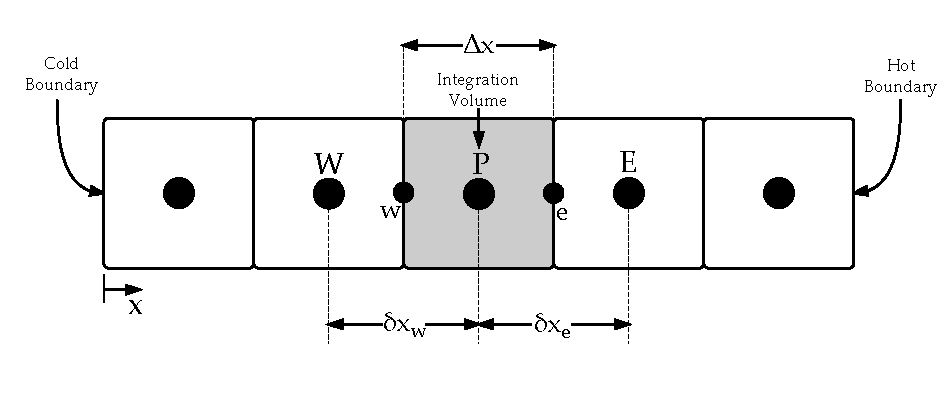
\includegraphics[scale=0.8]{1D_grid.pdf}
  \caption{Basic Cartesian grid for 1D domain.}
  \label{fig:1D_grid}
\end{figure}

\begin{equation}
\int_{t}^{t+\Delta t}\int_\mathrm{x_w}^\mathrm{x_e}\Biggl(\Psi\frac{\partial T}{\partial t} + \Lambda u \frac{\partial T}{\partial x}\Biggl)dxdt = \int_{t}^{t+\Delta t}\int_\mathrm{x_w}^\mathrm{x_e}\Biggl(\Gamma^{\phi} \frac{\partial^{2}T}{\partial x^2} + S^{\phi}\Biggl) dxdt
\label{1D_FVM1}
\end{equation}

After the integration, it is obtained:

\begin{equation}
\Psi[T_\mathrm{p}-T^0_\mathrm{p}]\Delta x +\Lambda u[T_\mathrm{e} - T_\mathrm{w}]\Delta t = \Gamma^{\phi}\Bigg[\Bigg(\frac{\partial T}{\partial x}\Bigg)_\mathrm{e}-\Bigg(\frac{\partial T}{\partial x}\Bigg)_\mathrm{w}\Bigg]\Delta t + S^{\phi}\Delta x\Delta t
\label{1D_FVM1_2}
\end{equation}

Table \ref{tab:EnEqVar} identifies the generic variables for the energy equations. Although only homogeneous meshes were evaluated in this work, the program was developed in a manner that allows $\Delta x$ to vary in the $x$ direction, resulting in non-linear meshes, which will be evaluated in further works.

\begin{table}[htp]\footnotesize
\caption{Variables in the energy equations.}
\label{tab:EnEqVar} 
\centering
\begin{tabular}{ccccc}
\toprule
Phase &  $\Psi$ & $\Lambda$ & $\Gamma^{\phi}$ & $S^{\phi}$\\\toprule
Solid  & $\rho_\textrm{s} c_\textrm{H}(1-\varepsilon)$ & 0 & $(1-\varepsilon)k_\textrm{s}^\textrm{eff}$ & $h \beta (T_\textrm{f}-T_\textrm{s}) + \dot{q}_\textrm{MCE}$\\\hline
{Fluid} &  {$\rho_\textrm{f} \varepsilon$} & {$\rho_\textrm{f} $} & $\varepsilon\bigl[\frac{k^\textrm{eff}_\textrm{f}}{c_\textrm{p,f}} + \rho_\textrm{f} D_{||}\bigr]$ & $\frac{h\beta}{c_\textrm{p,f}}(T_\textrm{s}-T_\textrm{f}) + \Biggl|\frac{u}{c_\textrm{p,f}}\frac{\partial P}{\partial x}\Biggr| + \dot{q}_\textrm{csg}$\\
\bottomrule
\end{tabular}
\end{table} 

\noindent where $\dot{q}_\textrm{csg}$ is only used when the wall heat transfer is considered and $\dot{q}_\textrm{MCE}$ is included when the built-in approach is used to simulate the MCE. Based on the discretized equations, the final numerical forms of each macroscopic balance will give a discretization in the following form:

\begin{equation}
a_pT_P = a_eT_E + a_wT_W + a_p^0T^0_P + b
\label{Gen_dis_eq}
\end{equation}

\subsubsection{Solid Energy Equation}
\label{sec:disc-solid}

The Central Difference Scheme (CDS) was used as the interpolating function for the diffusion terms. Thus:

%\nomenclature CDS

\begin{equation}
\frac{\partial T_\textrm{s}}{\partial x}\bigg|_\textrm{e} = \Biggl(\frac{T_\textrm{s,E}-T_\textrm{s,P}}{(\delta x)_\textrm{e}} \Biggr)
\end{equation}
\begin{equation}
\frac{\partial T_\textrm{s}}{\partial x}\bigg|_\textrm{w} = \Biggl(\frac{T_\textrm{s,P}-T_\textrm{s,W}}{(\delta x)_\textrm{w}} \Biggr)
\end{equation}

Using this interpolation scheme, the coefficients of Eq.~\eqref{Gen_dis_eq} are:

\begin{equation}
a_w = \frac{(1-\varepsilon)k_P}{(\delta x)_\textrm{w}} \nonumber
\end{equation}
\begin{equation}
a_e = \frac{(1-\varepsilon)k_P}{(\delta x)_\textrm{e}} \nonumber
\end{equation}
\begin{equation}
a_p^0 = \frac{(1-\varepsilon)\rho_\textrm{s} c_\textrm{H,P} \Delta x}{\Delta t} \nonumber
\end{equation}
\begin{equation}
a_{p,f} = h_\textrm{P}\beta \Delta x \nonumber
\end{equation}
\begin{equation}
b = a_{p,f}T_\textrm{f,P}+\dot{q}_\textrm{MCE}\Delta x \nonumber
\end{equation}
\begin{equation}
a_p = a_e + a_w + a_p^0 + a_{p,f} \nonumber
\end{equation}

For the boundary conditions, both boundaries are setted as adiabatic. Thus, $\frac{\partial T_\textrm{s}}{\partial x}(t,x^*=0)=\frac{\partial T_\textrm{s}}{\partial x}(t,x^*=1)=0$. The coefficients for these two volumes are the same as the ones presented above. The only difference is: $a_{w} = 0$ for the Cold or West boundary volume and $a_{e} = 0$ for the Hot or East boundary volume. For the initial condition, a linear temperature profile between $T_\textrm{C}$ and $T_\textrm{H}$ along the regenerator is assumed.

\nomenclature[galphai]{$\alpha^{i}$}{WUDS coefficient [\si{-}]}
\nomenclature[gbetai]{$\beta^{i}$}{WUDS coefficient [\si{-}]}

\subsubsection{Fluid Energy Equation}
\label{sec:disc-fluid}

A Weighted Upstream Differencing Scheme (WUDS) was adopted as the interpolation function for the advection and diffusion terms \cite{Maliska2004}, because the range of the Peclet number was evaluated, and it lies between 1 and 15. In this hybrid interpolation scheme two coefficients, $\alpha^{i}$ and $\beta^{i}$, are used as weight between advection and diffusion, depending on the Peclet number. This scheme was adopted, as no-flow conditions can exist in the AMR, and for this condition this scheme turns in the Central Difference Scheme (CDS). The coefficients $\alpha^{i}$ and $\beta^{i}$ are deduced analytically \cite{Maliska2004}, but in this work it is used the expression proposed by \cite{Raithby}, since these coefficients are not in the exponential form, resulting in lower computational cost. The numerical interpolations for Eq.~\eqref{1D_FVM1_2} of the advective and diffusive terms are, respectively:

\begin{equation}
T_\textrm{f,e}= (0.5+\alpha^{i}_P)T_\textrm{f,P}+(0.5-\alpha^{i}_P)T_\textrm{f,E}
\end{equation}
\begin{equation}
T_\textrm{f,w}= (0.5+\alpha^{i}_P)T_\textrm{f,W}+(0.5-\alpha^{i}_P)T_\textrm{f,P}
\end{equation}

\begin{equation}
\frac{\partial T_\textrm{f}}{\partial x}\bigg|_\textrm{e} = \beta^{i}_P\Biggl(\frac{T_\textrm{f,E}-T_\textrm{f,P}}{(\delta x)_\textrm{e}} \Biggr)
\end{equation}
\begin{equation}
\frac{\partial T_\textrm{f}}{\partial x}\bigg|_\textrm{w} = \beta^{i}_P\Biggl(\frac{T_\textrm{f,P}-T_\textrm{f,W}}{(\delta x)_\textrm{w}} \Biggr)
\end{equation}

\noindent where $\alpha^{i}$ and $\beta^{i}$ are given by:

\begin{equation}
\alpha^{i}_\textrm{P} = \frac{Pe_P^2}{10+2Pe_P^2}
\label{WUDS_alpha}
\end{equation}
\begin{equation}
\beta^{i}_\textrm{P} = \frac{1+0.005Pe_P^2}{1+0.05Pe_P^2}
\label{WUDS_beta}
\end{equation}

\noindent and $Pe_P$ is defined by:

\begin{equation}
Pe_P = \frac{\rho_\textrm{P}c_\textrm{p,P}u}{\varepsilon\bigl(k_\textrm{P} + \rho_\textrm{P} c_\textrm{p,P}D_\textrm{||,P}\bigr)} \Delta x
\label{WUDS_Pe}
\end{equation}

Using this interpolation scheme, the coefficients of Eq.~\eqref{Gen_dis_eq} are: 

\nomenclature[ib]{$\textrm{b}$}{Boundary}
\nomenclature[ipresc]{$\textrm{presc}$}{Prescribed}
\nomenclature[i_1]{$*$}{Represents non-dimensional variables}
\nomenclature[vtdma]{TDMA}{Tri-Diagonal Matrix Algorithm}
\nomenclature[iamb]{$\textrm{amb}$}{Ambient}
\nomenclature[isur]{$\textrm{sur}$}{Surroundings}
\nomenclature[cf]{$f_\textrm{i}$}{Interpolation factor [\si{-}]}
\nomenclature[as]{$s$}{Entropy [\si{J/kg-K}]}

$$
a_e= \rho_\textrm{P} u_\textrm{P} (-0.5+\alpha_\textrm{P}) +\frac{\varepsilon (\frac{k_P}{c_\textrm{p,P}}+\rho_P D_{||,P})}{(\delta x)_e}\beta_\textrm{P}
$$

$$
a_w = \rho_\textrm{P} u_\textrm{P} (0.5+\alpha_\textrm{P}) +\frac{\varepsilon (\frac{k_\textrm{P}}{c_\textrm{p,P}}+\rho D_\textrm{||,P})}{(\delta x)_w}\beta_\textrm{P}
$$

$$
ap^0 = \frac{\varepsilon\rho_\textrm{P}\Delta x}{\Delta t}
$$

$$
a_{p,f} = \frac{h_\textrm{P}\beta\Delta x}{c_\textrm{p,P}} 
$$

$$
b = a_{p,f}T_s + \left| \frac{u_\textrm{P}\Delta x}{c_\textrm{p,P}}\frac{\partial P}{\partial x}\right| + \dot{q}_\textrm{csg}\frac{\Delta x}{c_\textrm{p,P}}
$$

$$
a_p = a_p^0 + a_{p,f} + a_e + a_w 
$$

For the fluid energy equation, the boundary conditions depend on the direction of fluid flow and are described in Table \ref{tab:fluid-bc}, where $T_\textrm{b}$ is the domain boundary temperature and $T_\textrm{presc}$ is a prescribed temperature. The coefficients for the west and east volume are described in Table \ref{tab:fluid-coef-bc}.

\begin{table}[htp]
\centering
\caption{Fluid boundary conditions.}
\label{tab:fluid-bc}
\begin{tabular}{c|c|c|ll}
\cline{2-3}
\multicolumn{1}{l|}{}       & Cold or West boundary                                  & Hot or East boundary                                  &  &  \\ \cline{1-3}
\multicolumn{1}{|c|}{$u>0$} & $T_\textrm{b} = T_\textrm{presc}$                      & $\frac{\partial T_\textrm{f}}{\partial x}(t,x^*=1)=0$ &  &  \\ \cline{1-3}
\multicolumn{1}{|c|}{$u<0$} & $\frac{\partial T_\textrm{f}}{\partial x}(t,x^*=0) =0$ & $T_\textrm{b} = T_\textrm{presc}$                     &  &  \\ \cline{1-3}
\multicolumn{1}{|c|}{$u=0$} & $\frac{\partial T_\textrm{f}}{\partial x}(t,x^*=0)=0$  & $\frac{\partial T_\textrm{f}}{\partial x}(t,x^*=1)=0$ &  &  \\ \cline{1-3}
\end{tabular}
\end{table}

\begin{table}[htp]
\centering
\caption{Coefficients for the fluid boundary conditions.}
\label{tab:fluid-coef-bc}
\begin{tabular}{c|c|c|ll}
\cline{2-3}
\multicolumn{1}{l|}{}       & Cold or West boundary                                                                                                                                                                                                                                                                                                                                                                                                                                                                                                                                                   & Hot or East boundary                                                                                                                                                                                                                                                                                                                                                                                                                                                                                                                                                     &  &  \\ \cline{1-3}
\multicolumn{1}{|c|}{$u>0$} & \begin{tabular}[c]{@{}c@{}}$a_e= \rho u \lvert_e (-0.5+\alpha_p) +\frac{\varepsilon (\frac{k}{c_p}+\rho D_{||})}{\delta x_e}\beta_p$\\ $a_{w,f} = \frac{\varepsilon (\frac{\kappa}{c_p}+\rho D_{||})}{\Delta x/2}+\rho u$\\ $ap^0 = \frac{\varepsilon\rho\Delta x}{\Delta t}$\\ $a_{p,f} = \frac{h\beta\Delta x}{c_p} $\\ $b = a_{p,f}T_s + \left| \frac{u\Delta x}{c_p}\frac{\partial P}{\partial x}\right| + \dot{q}_\textrm{csg}\frac{\Delta x}{c_p}+a_{w,f}T_{pres}$\\ $a_p = a_p^0 + a_{p,f} + a_e + a_{w,f} - \rho u \lvert_w +\rho u \lvert_e$\end{tabular} & \begin{tabular}[c]{@{}c@{}}$a_e=0$\\ $a_w = \rho u \lvert_w (0.5+\alpha_p) +\frac{\varepsilon (\frac{\kappa}{c_p}+\rho D_{||})}{\delta x_w}\beta_p$\\ $ap^0 = \frac{\varepsilon\rho\Delta x}{\Delta t}$\\ $a_{p,f} = \frac{h\beta\Delta x}{c_p} $\\ $b = a_{p,f}T_s + \left| \frac{u\Delta x}{c_p}\frac{\partial P}{\partial x}\right| + \dot{q}_\textrm{csg}\frac{\Delta x}{c_p}$\\ $a_p = a_p^0 + a_{p,f} + a_e + a_w - \rho u \lvert_w +\rho u \lvert_e$\end{tabular}                                                                                                 &  &  \\ \cline{1-3}
\multicolumn{1}{|c|}{$u<0$} & \begin{tabular}[c]{@{}c@{}}$a_e= \rho u \lvert_e (-0.5+\alpha_p) +\frac{\varepsilon (\frac{\kappa}{c_p}+\rho D_{||})}{\delta x_e}\beta_p$\\ $a_w = 0$\\ $ap^0 = \frac{\varepsilon\rho\Delta x}{\Delta t}$\\ $a_{p,f} = \frac{h\beta\Delta x}{c_p} $\\ $b = a_{p,f}T_s + \left| \frac{u\Delta x}{c_p}\frac{\partial P}{\partial x}\right| + \dot{q}_\textrm{csg}\frac{\Delta x}{c_p}$\\ $a_p = a_p^0 + a_{p,f} + a_e + a_w - \rho u \lvert_w +\rho u \lvert_e$\end{tabular}                                                                                              & \begin{tabular}[c]{@{}c@{}}$a_{e,f}= \frac{\varepsilon (\frac{\kappa}{c_p}+\rho D_{||})}{\Delta x/2}-\rho u$\\ $a_w = \rho u \lvert_w (0.5+\alpha_p) +\frac{\varepsilon (\frac{\kappa}{c_p}+\rho D_{||})}{\delta x_w}\beta_p$\\ $ap^0 = \frac{\varepsilon\rho\Delta x}{\Delta t}$\\ $a_{p,f} = \frac{h\beta\Delta x}{c_p} $\\ $b = a_{p,f}T_s + \left| \frac{u\Delta x}{c_p}\frac{\partial P}{\partial x}\right| + \dot{q}_\textrm{csg}\frac{\Delta x}{c_p}+a_{e,f}T_{pres}$\\ $a_p = a_p^0 + a_{p,f} + a_{e,f} + a_{w} - \rho u \lvert_w +\rho u \lvert_e$\end{tabular} &  &  \\ \cline{1-3}
\multicolumn{1}{|c|}{$u=0$} & \begin{tabular}[c]{@{}c@{}}$a_e= \rho u \lvert_e (-0.5+\alpha_p) +\frac{\varepsilon (\frac{\kappa}{c_p}+\rho D_{||})}{\delta x_e}\beta_p$\\ $a_w = 0$\\ $ap^0 = \frac{\varepsilon\rho\Delta x}{\Delta t}$\\ $a_{p,f} = \frac{h\beta\Delta x}{c_p} $\\ $b = a_{p,f}T_s + \left| \frac{u\Delta x}{c_p}\frac{\partial P}{\partial x}\right| + \dot{q}_\textrm{csg}\frac{\Delta x}{c_p}$\\ $a_p = a_p^0 + a_{p,f} + a_e + a_w - \rho u \lvert_w +\rho u \lvert_e$\end{tabular}                                                                                              & \begin{tabular}[c]{@{}c@{}}$a_e=0$\\ $a_w = \rho u \lvert_w (0.5+\alpha_p) +\frac{\varepsilon (\frac{\kappa}{c_p}+\rho D_{||})}{\delta x_w}\beta_p$\\ $ap^0 = \frac{\varepsilon\rho\Delta x}{\Delta t}$\\ $a_{p,f} = \frac{h\beta\Delta x}{c_p} $\\ $b = a_{p,f}T_s + \left| \frac{u\Delta x}{c_p}\frac{\partial P}{\partial x}\right| + \dot{q}_\textrm{csg}\frac{\Delta x}{c_p}$\\ $a_p = a_p^0 + a_{p,f} + a_e + a_w - \rho u \lvert_w +\rho u \lvert_e$\end{tabular}                                                                                                 &  &  \\ \cline{1-3}
\end{tabular}
\end{table}

The solver for the energy equations is a line-by-line Tri-Diagonal Matrix Algorithm (TDMA). This designation refers to the fact that when the matrix of the coefficients of these equations is written, all the nonzero coefficients align themselves along three diagonals of the matrix. This solver, also known as the Thomas Algorithm, was chosen because it requires computer storage and computer time proportional only to $N$ (volumes), rather than to $N^2$ or $N^3$, as other methods \cite{Patankar1980}. For the initial condition, a linear temperature profile between $T_\textrm{C}$ and $T_\textrm{H}$ along the regenerator is assumed.

Since the fluid and the solid energy are solved coupled, there is an initial guess  for the temperature profiles. For any given time, the fluid equation is solved first, and its solution is used to solve the solid energy equation. This process is repeated until the convergence criteria is satisfied, that will be defined in Section \ref{subsec:conv-crit}.

\subsection{Casing Energy Equation}
\label{sec:disc-casing}

The casing energy equation is also discretized using a fully implicit scheme. Fig. \ref{fig:2D_grid} represents the two dimensional domain of the casing. Eq.~\eqref{EnergyEquation_Casing} is discretized  by the integration in time , x and y direction, using a fully implicit scheme. Thus:

\begin{figure}[!ht]
  \centering
  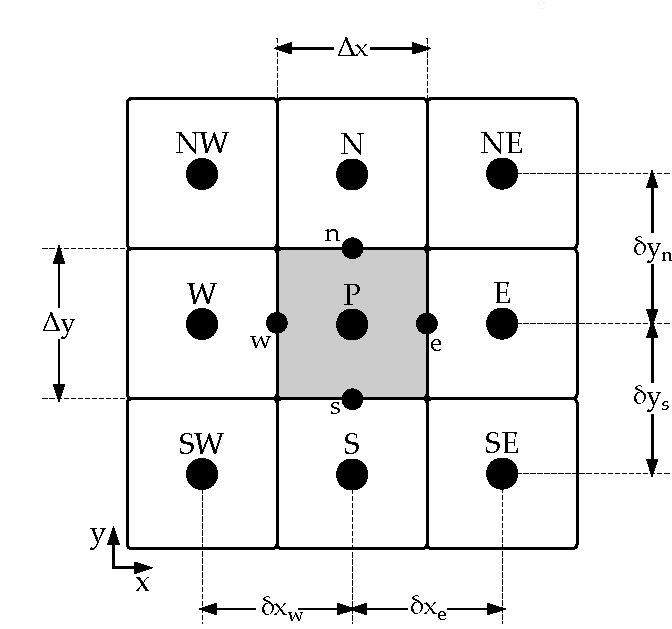
\includegraphics[scale=0.8]{2D_grid.pdf}
  \caption{Basic Cartesian grid for 2D domain.}
  \label{fig:2D_grid}
\end{figure}

\begin{equation}
\int_{t}^{t+\Delta t}\int_\mathrm{y_s}^\mathrm{y_n}\int_\mathrm{x_w}^\mathrm{x_e} \rho_\textrm{csg} c_\mathrm{p,csg}\frac{\partial T_\textrm{csg}}{\partial t}dxdydt = \int_{t}^{t+\Delta t}\int_\mathrm{y_s}^\mathrm{y_n}\int_\mathrm{x_w}^\mathrm{x_e}\frac{\partial}{\partial y}\Bigg(k_\mathrm{y}\frac{\partial T_\textrm{csg}}{\partial y}\Bigg) dxdy dt + \nonumber
\end{equation}
\begin{equation}
\int_{t}^{t+\Delta t}\int_\mathrm{y_s}^\mathrm{y_n}\int_\mathrm{x_w}^\mathrm{x_e}\frac{\partial}{\partial x}\Bigg(k_\mathrm{x}\frac{\partial T_\textrm{csg}}{\partial x}\Bigg)dxdy dt
\label{2D_disc}
\end{equation}

After the integration, Eq.~\eqref{2D_disc} results in:

\begin{equation}
\rho_\textrm{csg} c_\mathrm{p,csg}[T_p-T^0_p]\Delta x \Delta y = \Bigg[\Bigg(k_\mathrm{y}\frac{\partial T_\textrm{csg}}{\partial y}\Bigg)_\mathrm{y_n}-\Bigg(k_\mathrm{y}\frac{\partial T_\textrm{csg}}{\partial y}\Bigg)_\mathrm{y_s}\Bigg] \Delta x \Delta t + \nonumber 
\end{equation}
\begin{equation}
\Bigg[\Bigg(k_\mathrm{x}\frac{\partial T_\textrm{csg}}{\partial x}\Bigg)_\mathrm{x_e}-\Bigg(k_\mathrm{x}\frac{\partial T_\textrm{csg}}{\partial x}\Bigg)_\mathrm{x_w}\Bigg] \Delta y \Delta t
\label{2D_disc_2}
\end{equation}

Using the CDS interpolation scheme and dividing Eq.~\eqref{2D_disc_2} by $\Delta t$:

\begin{equation}
\frac{\rho_\textrm{csg} c_\mathrm{p,csg}\Delta x \Delta y}{\Delta t}[T_p-T^0_p] = \Bigg[\frac{k_\mathrm{y,n}\Delta x}{(\delta y)_\mathrm{n}}\big(T_\mathrm{N}-T_\mathrm{P}\big) -\frac{k_\mathrm{y,s}\Delta x}{(\delta y)_\mathrm{s}}\big(T_\mathrm{P}-T_\mathrm{S}\big)\Bigg] +
\nonumber 
\end{equation}
\begin{equation}
\Bigg[\frac{k_\mathrm{x,e}\Delta y}{(\delta x)_\mathrm{e}}\big(T_\mathrm{E}-T_\mathrm{P}\big) -\frac{k_\mathrm{x,w}\Delta y}{(\delta x)_\mathrm{w}}\big(T_\mathrm{P}-T_\mathrm{W}\big)\Bigg]
\label{2D_disc_3}
\end{equation}

Although the casing energy equation is written in the conservative form, it was assumed constant properties within the volume domain, being unnecessary to evaluate the properties at the boundaries of the volume. Since the casing contains two materials, i.e. wall and air, the thermal conductivity at the material's interface must be evaluated. It is important to emphasize that one volume never contains two materials. Therefore, a non-homogeneous grid spacing can be generated. The thermal conductivity in the interface of two different materials is evaluated as:

\begin{equation}
k_\mathrm{y,n} = \Bigg(\frac{1-f_\textrm{i}}{k_\mathrm{y,P}} + \frac{f_\textrm{i}}{k_\mathrm{y,E}}\Bigg)
\label{k_evaluation}
\end{equation}

\noindent where $f_\textrm{i}$ is the interpolation factor defined in terms of the distances shown in Fig. \ref{fig:kn_evaluation}.

\begin{equation}
f_\textrm{i} =\frac{\delta y_\mathrm{n+}}{\delta y_\mathrm{n}}
\end{equation}

\begin{figure}[!ht]
  \centering
  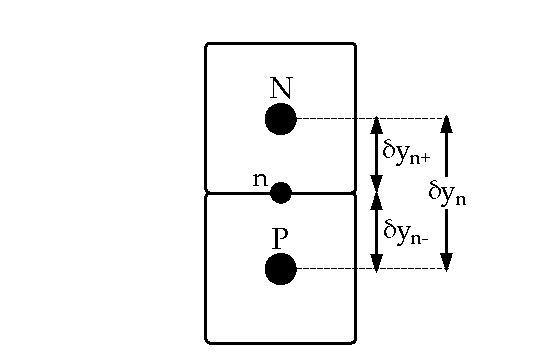
\includegraphics[scale=0.8]{kn_evaluation.pdf}
  \caption{Distances associated with the interface $\mathrm{n}$.}
  \label{fig:kn_evaluation}
\end{figure}

It is possible to rearrange the terms of equation Eq.~\eqref{2D_disc_3} as:

\begin{equation}
a_pT_P = a_eT_E + a_wT_W + a_nT_N + a_sT_S +a_p^0T_P^0 +b
\label{2D-general}
\end{equation}

\noindent where:

\begin{equation}
a_w = \frac{k_\mathrm{x,w}\Delta y}{(\delta x)_\mathrm{w}}  \nonumber
\end{equation}
\begin{equation}
a_e = \frac{k_\mathrm{x,e}\Delta y}{(\delta x)_\mathrm{e}} \nonumber
\end{equation}
\begin{equation}
a_s = \frac{k_\mathrm{y,s}\Delta x}{(\delta y)_\mathrm{s}} \nonumber
\end{equation}
\begin{equation}
a_n = \frac{k_\mathrm{y,n}\Delta x}{(\delta y)_\mathrm{n}} \nonumber
\end{equation}
\begin{equation}
a_p^0 = \frac{\rho_\textrm{csg} c_\textrm{p,csg} \Delta x \Delta y}{\Delta t}  \nonumber
\end{equation}
\begin{equation}
b = 0 \nonumber
\end{equation}
\begin{equation}
a_p = a_p^0 + a_e + a_w + a_n + a_s \nonumber
\end{equation}

For the boundaries conditions, the West and East boundaries are setted as adiabatic. Thus, $\frac{\partial T_\textrm{csg}(t,x^{*}=0,y)}{\partial x} = \frac{\partial T_\textrm{csg}(t,x^{*}=1,y)}{\partial x} = 0$. The South boundary is in contact with the porous medium, thus a prescribed flux condition is employed, according to Eq.~\eqref{Q_HTwall}, since it is considered that the solid spheres have infinitesimal contact area with the casing and consequently, the solid and casing domains do not interact. For the North boundary condition, it is assumed that the magnetic circuit has a very large thermal inertia and its temperature is equal to that of the ambient. Therefore, it is used a prescribed temperature for this boundary, $T_\textrm{pres} = T_\textrm{amb}$, where $T_\textrm{amb}$ is the ambient temperature. Thus, the coefficients for all boundaries are:

West boundary:
\begin{equation}
a_w = 0 \nonumber
\end{equation}
\begin{equation}
a_e = \frac{k_\mathrm{x,e}\Delta y}{(\delta x)_\mathrm{e}} \nonumber
\end{equation}
\begin{equation}
a_s = \frac{k_\mathrm{y,s}\Delta x}{(\delta y)_\mathrm{s}} \nonumber
\end{equation}
\begin{equation}
a_n = \frac{k_\mathrm{y,n}\Delta x}{(\delta y)_\mathrm{n}} \nonumber
\end{equation}
\begin{equation}
a_p^0 = \frac{\rho_\textrm{csg} c_\textrm{p,csg} \Delta x \Delta y}{\Delta t}  \nonumber
\end{equation}
\begin{equation}
b = 0 \nonumber
\end{equation}
\begin{equation}
a_p = a_p^0 + a_e + a_w + a_n + a_s \nonumber
\end{equation}

East boundary:
\begin{equation}
a_w = \frac{k_\mathrm{x,w}\Delta y}{(\delta x)_\mathrm{w}}  \nonumber
\end{equation}
\begin{equation}
a_e = 0 \nonumber
\end{equation}
\begin{equation}
a_s = \frac{k_\mathrm{y,s}\Delta x}{(\delta y)_\mathrm{s}} \nonumber
\end{equation}
\begin{equation}
a_n = \frac{k_\mathrm{y,n}\Delta x}{(\delta y)_\mathrm{n}} \nonumber
\end{equation}
\begin{equation}
a_p^0 = \frac{\rho_\textrm{csg} c_\textrm{p,csg} \Delta x \Delta y}{\Delta t}  \nonumber
\end{equation}
\begin{equation}
b = 0 \nonumber
\end{equation}
\begin{equation}
a_p = a_p^0 + a_e + a_w + a_n + a_s \nonumber
\end{equation}

South boundary:
\begin{equation}
a_w = \frac{k_\mathrm{x,w}\Delta y}{(\delta x)_\mathrm{w}}  \nonumber
\end{equation}
\begin{equation}
a_e = \frac{k_\mathrm{x,e}\Delta y}{(\delta x)_\mathrm{e}} \nonumber
\end{equation}
\begin{equation}
a_s = 0 \nonumber
\end{equation}
\begin{equation}
a_n = \frac{k_\mathrm{y,n}\Delta x}{(\delta y)_\mathrm{n}} \nonumber
\end{equation}
\begin{equation}
a_p^0 = \frac{\rho_\textrm{csg} c_\textrm{p,csg} \Delta x \Delta y}{\Delta t}  \nonumber
\end{equation}
\begin{equation}
b = q''_\textrm{presc}\Delta x \nonumber
\end{equation}
\begin{equation}
a_p = a_p^0 + a_e + a_w + a_n + a_s \nonumber
\end{equation}

North boundary:
\begin{equation}
a_w = \frac{k_\mathrm{x,w}\Delta y}{(\delta x)_\mathrm{w}}  \nonumber
\end{equation}
\begin{equation}
a_e = \frac{k_\mathrm{x,e}\Delta y}{(\delta x)_\mathrm{e}} \nonumber
\end{equation}
\begin{equation}
a_s = \frac{k_\mathrm{y,s}\Delta x}{(\delta y)_\mathrm{s}} \nonumber
\end{equation}
\begin{equation}
a_n = 0 \nonumber
\end{equation}
\begin{equation}
a_{n,f} = \frac{k_\mathrm{y,n}\Delta x}{\Delta y/2} \nonumber
\end{equation}
\begin{equation}
a_p^0 = \frac{\rho_\textrm{csg} c_\textrm{p,csg} \Delta x \Delta y}{\Delta t}  \nonumber
\end{equation}
\begin{equation}
b = a_{n,f}T_\textrm{amb} \nonumber
\end{equation}
\begin{equation}
a_p = a_p^0 + a_e + a_w + a_{n,f} + a_s \nonumber
\end{equation}

Numerically, the prescribed flux of the south boundary is given by:
\begin{equation}
q''_\textrm{presc} = \frac{h_\textrm{csg}}{1+\frac{h_\textrm{csg}\Delta y/2}{k_\textrm{y,csg}}}(T_\textrm{f}(t,x)-T_\textrm{f}(t,x,y=\Delta y/2))
\end{equation}

\noindent for a flow condition and:

\begin{equation}
q''_\textrm{presc} = 0
\end{equation}

\noindent for a no-flow condition.

The four domain edge volumes coefficients are the combination of the boundaries that are in contact. The initial temperature guess is linear in $x$ and $y$ directions. The TDMA solver is also used for the casing energy equation, but with an additional convergence loop for the $y$ direction. Thus, convergence is obtained when two successive iterations satisfy the following criterion:

\begin{equation}
\textrm{Max} \bigg| T_\textrm{(csg)}(t,x,y)| - T_\textrm{(csg)}(t,x,y)|^{**} \bigg| < 10^\textrm{-6} 
\end{equation}

\noindent where the superscript $**$ refers to the previous iteration. The value of 10$^{-6}$ is suggested by \cite{Trevizoli2015}. The casing heat transfer model is solved coupled with the fluid and solid porous medium energy equations, as will be detailed in Section \ref{sec:solver-routine}.

\nomenclature[i_2]{$**$}{Previous iteration}

\subsection{Multilayer Implementation?}

\textcolor{red}{Colocar propriedades dos materiais?}

\textcolor{red}{colocar no apendice rotina de solucao}



\section{Energy Conservation}
\textcolor{red}{mesh validation?}

Considering the FVM, the equations are obtained from energy balances in each elemental volume. Thus, the energy must be conserved in both volume and domain levels \cite{Maliska2004}. In this section, the energy balance in the domain level is verified, as a post processing, in order to validate the FVM implementation. The energy balance for solid, fluid and casing domain is described, then the results are showed. For all domains, the balance is given by:

\begin{equation}
\label{En_bal_general}
\dot{E}_\textrm{in} - \dot{E}_\textrm{out} + \dot{E}_\textrm{g} = \dot{E}_\textrm{st}
\end{equation}

\noindent where $\dot{E}_\textrm{in}$ is the energy that enters to the domain, $\dot{E}_\textrm{out}$ is the energy that exits the domain, $\dot{E}_\textrm{g}$ is the energy generate in the domain and $\dot{E}_\textrm{st}$ is the stored energy. For practicality, the fluid flow profile used in this analysis is an instantaneous profile and the magnetic profile is the same as the defined in Fig. \ref{fig:Trevizoli_magnet}.

\subsection{Solid Domain}
Since the solid domain boundary is setted as adiabatic, the only energy that enters or exits the domain is due to convection, $q_\textrm{conv}$, with the fluid phase. For AMRs, the MCE is an energy generation term, $\dot{q}_\textrm{MCE}$. The energy storage, $q_\textrm{tran}$, is represented by the transient term. These terms are quantified by:

\begin{equation}
\label{EC_s_conv}
q_\textrm{conv} =\sum_{x=1}^{N_x} h(x)A_\textrm{c}\beta \big(T_\textrm{f}(x) - T_\textrm{s}(x)\bigg) \Delta x(x)
\end{equation}

\begin{equation}
\label{EC_s_trans}
q_\textrm{tran} = \sum_{x=1}^{N_x} \rho_\textrm{s}c_\textrm{H}(x)\big(1-\varepsilon\big)A_\textrm{c} \Delta x(x) \frac{T_\textrm{s}(x) - T_\textrm{s}^0(x)}{\Delta t}
\end{equation}

\begin{equation}
\label{EC_s_mce}
\dot{q}_\textrm{MCE} = \sum_{x=1}^{N_x} -\rho_\textrm{s}\big(1-\varepsilon\big)A_\textrm{c} \Delta x(x) T_\textrm{s}(x)\frac{\partial s}{\partial B}\frac{\partial B}{\partial t}
\end{equation}

The results for the implementation of these equations are presented in Fig. \ref{fig:CE_solid_1} for the parameters of AMR 1 summarized in Table \ref{tab:mesh_cases}.

\begin{figure}[!ht]
  \centering
  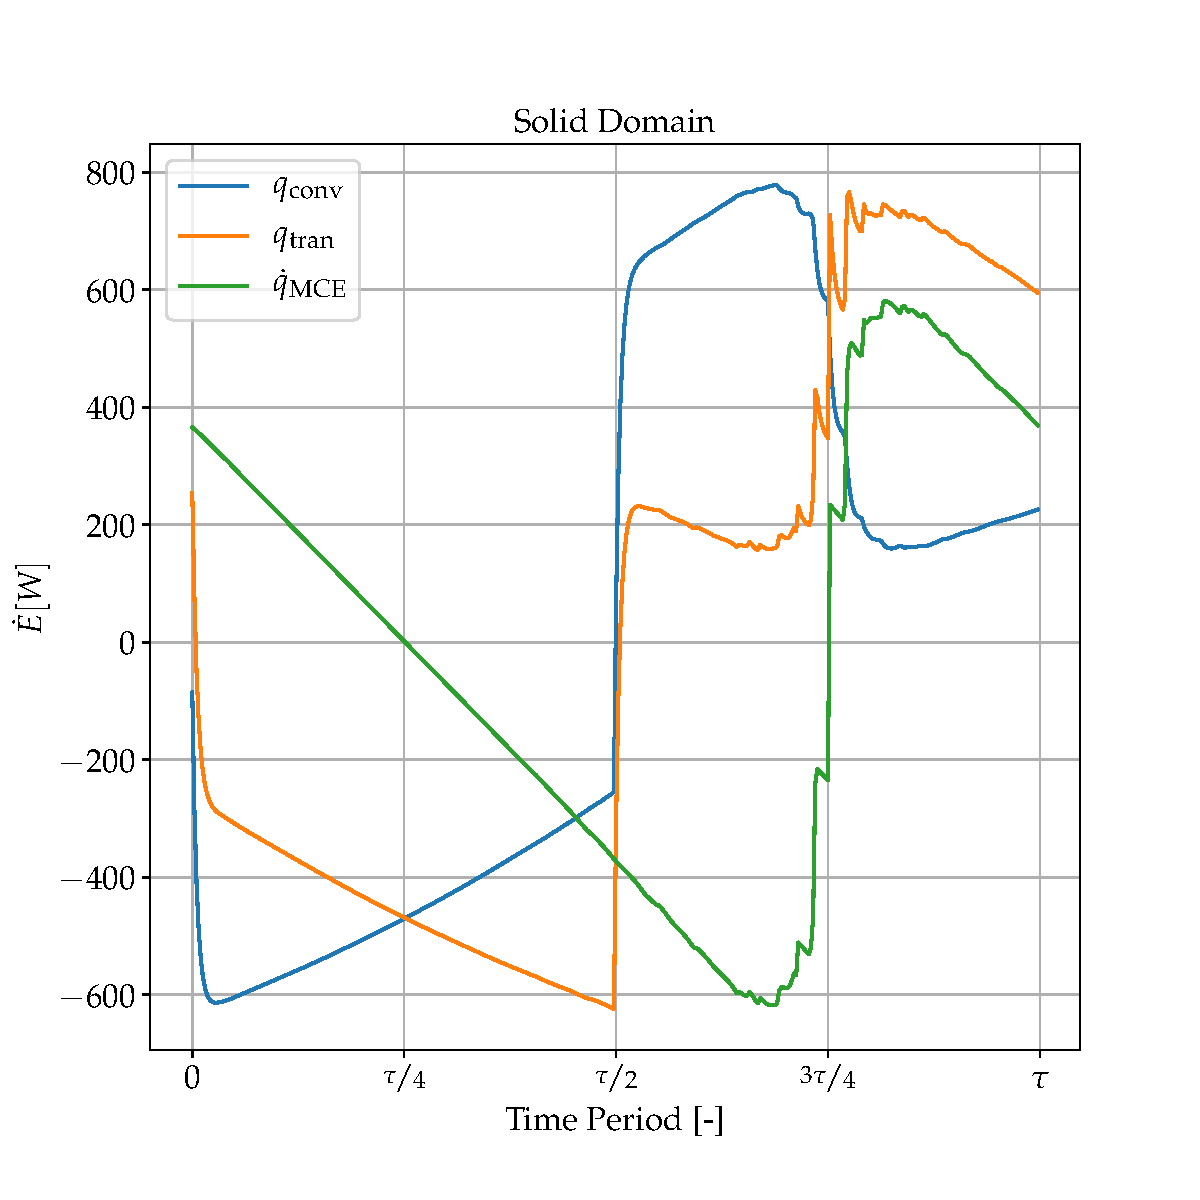
\includegraphics[scale=0.6]{CE_solid_1.pdf}
  \caption{Energy balance for the solid domain, using the parameters of AMR 1 given in Table \ref{tab:mesh_cases}.}
  \label{fig:CE_solid_1}
\end{figure}

The green curve of Fig. \ref{fig:CE_solid_1} is a reflection of the time derivative of the rectified cosine waveform, as can be inferred from Eq.~\eqref{EC_s_mce}. The horizontal axis exhibits the dimensionless time period, $\tau$. The times $\nicefrac{\tau}{4}$ and $\nicefrac{3\tau}{4}$ are the maximum and minimum magnetic field instants, respectively. The fluctuations that occurs in $\dot{q}_\textrm{MCE}$ (and further are transmitted for the other heat fluxes), can be explained by the non-linearities of the demagnetization field combined with the non-linear axial temperature profile, which is in the ferromagnetic phase near the cold end, and in the paramagnetic phase near the hot end. Although these fluctuations are occurring, they do not disturb the results or the analysis. The time between $0$ and $\nicefrac{\tau}{2}$ represents the CB, while the time between $\nicefrac{\tau}{2}$ and $\tau$ represents the HB. The convection heat flux varies according to the blows. During the CB, the solid phase gives heat to the fluid phase, while in the HB, the solid phase receives heat from the fluid phase. The transient heat can be understood as the outcome of the two other fluxes. Rewriting the sum of these fluxes, as given by Eq.~\eqref{En_bal_general}, it is obtained:

\begin{equation}
\label{En_bal_s}
q_\textrm{conv} + \dot{q}_\textrm{MCE} - q_\textrm{tran} = 0
\end{equation}

Fig. \ref{fig:CE_solid_2} (a) represents Eq.~\eqref{En_bal_s} graphically. In the FVM, the sum of the fluxes must be zero. As can be seen in the figure, except for $t = 0$, the sum of the energy balance is very close to zero. In the initial time, the energy residue of the balance, approximately -25 W, represents an absolute error of 4\%, considering the order of magnitude of the heat flux of 600 W as pointed in Fig. \ref{fig:CE_solid_1}. Although it seems that the initial time has an energy sink, this value is compensated by the fluid phase, as it will be presented in Section \ref{subsec:Fluid_domain}. This response is explained by the insufficient coupling of the solid and fluid equations, which the convergence criteria was defined in Section \ref{subsec:conv-crit} as $\varepsilon_\textrm{cycle}= 10^{-3}$ and $\varepsilon_\textrm{conv} = 10^{-4}$. Fig. \ref{fig:CE_solid_2} (b) shows the results for the same energy balance, but using a smaller convergence criteria, $\varepsilon_\textrm{cycle}= \varepsilon_\textrm{conv}$ = 10$^{-8}$. It can be noticed that the absolute error has significantly decreased, albeit it has not yet reached zero. A perfect balance would only be achieve with a perfect coupling of the domains, which in practice is unworkable.

\begin{figure}[!ht]
  \centering
  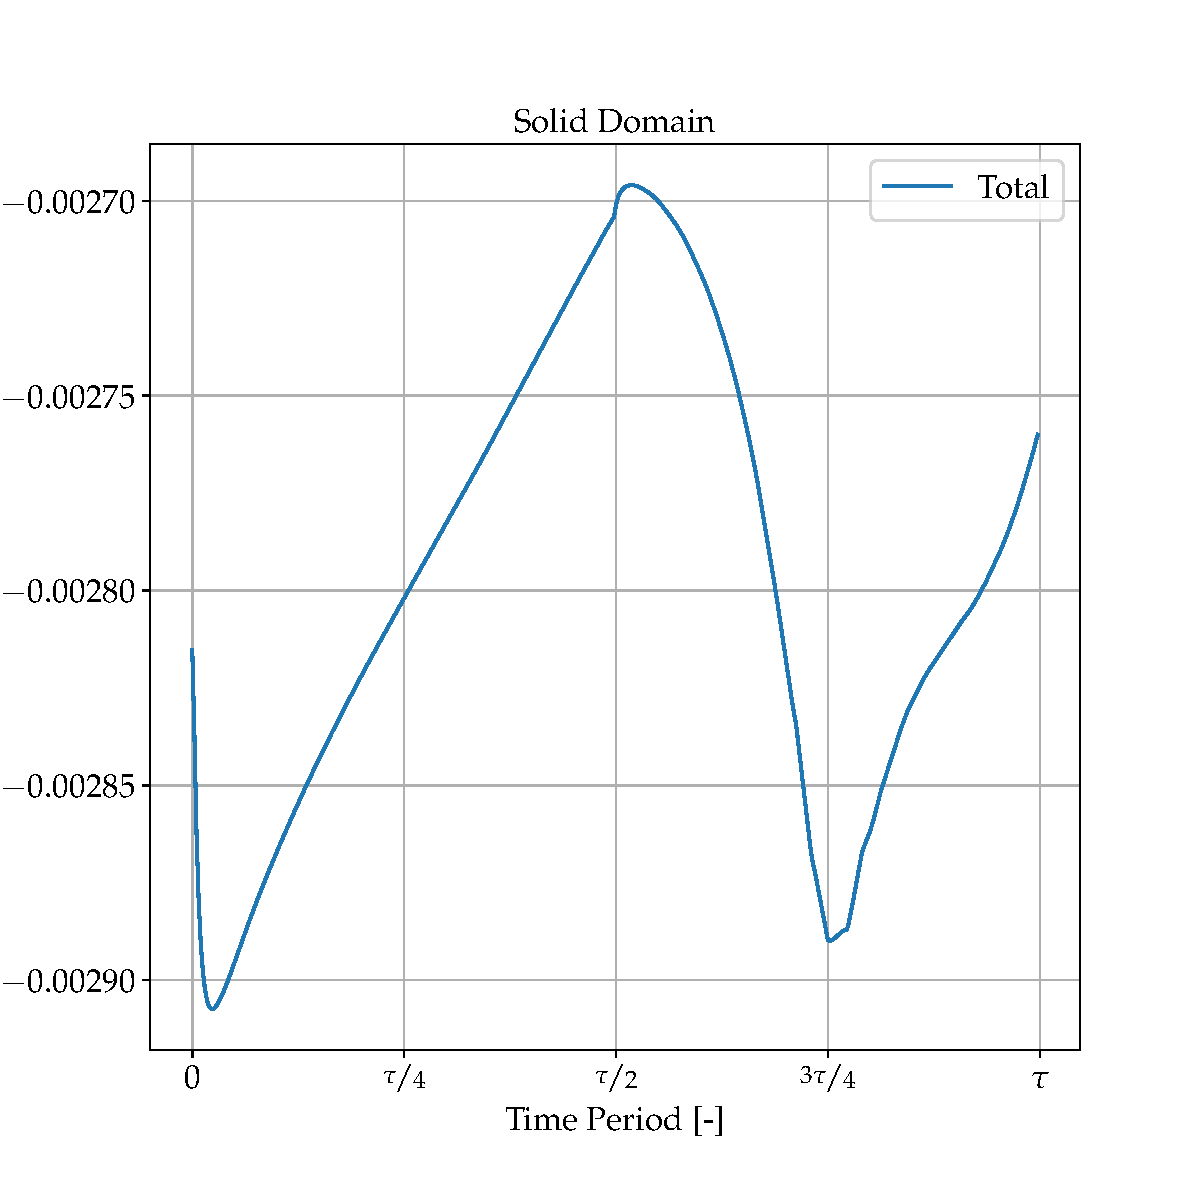
\includegraphics[scale=0.6]{CE_solid_3.pdf}
  \caption{Sum of the heat fluxes as pointed by Eq.~\eqref{En_bal_s}: (a) Using the criteria defined in Section \ref{subsec:conv-crit} ($\varepsilon_\textrm{cycle}= 10^{-3}$ and $\varepsilon_\textrm{conv} = 10^{-4}$) and; (b) Using the criteria $\varepsilon_\textrm{cycle}= \varepsilon_\textrm{conv} = 10^{-8}$.}
  \label{fig:CE_solid_2}
\end{figure}

\subsection{Fluid Domain}

\begin{figure}[!ht]
  \centering
  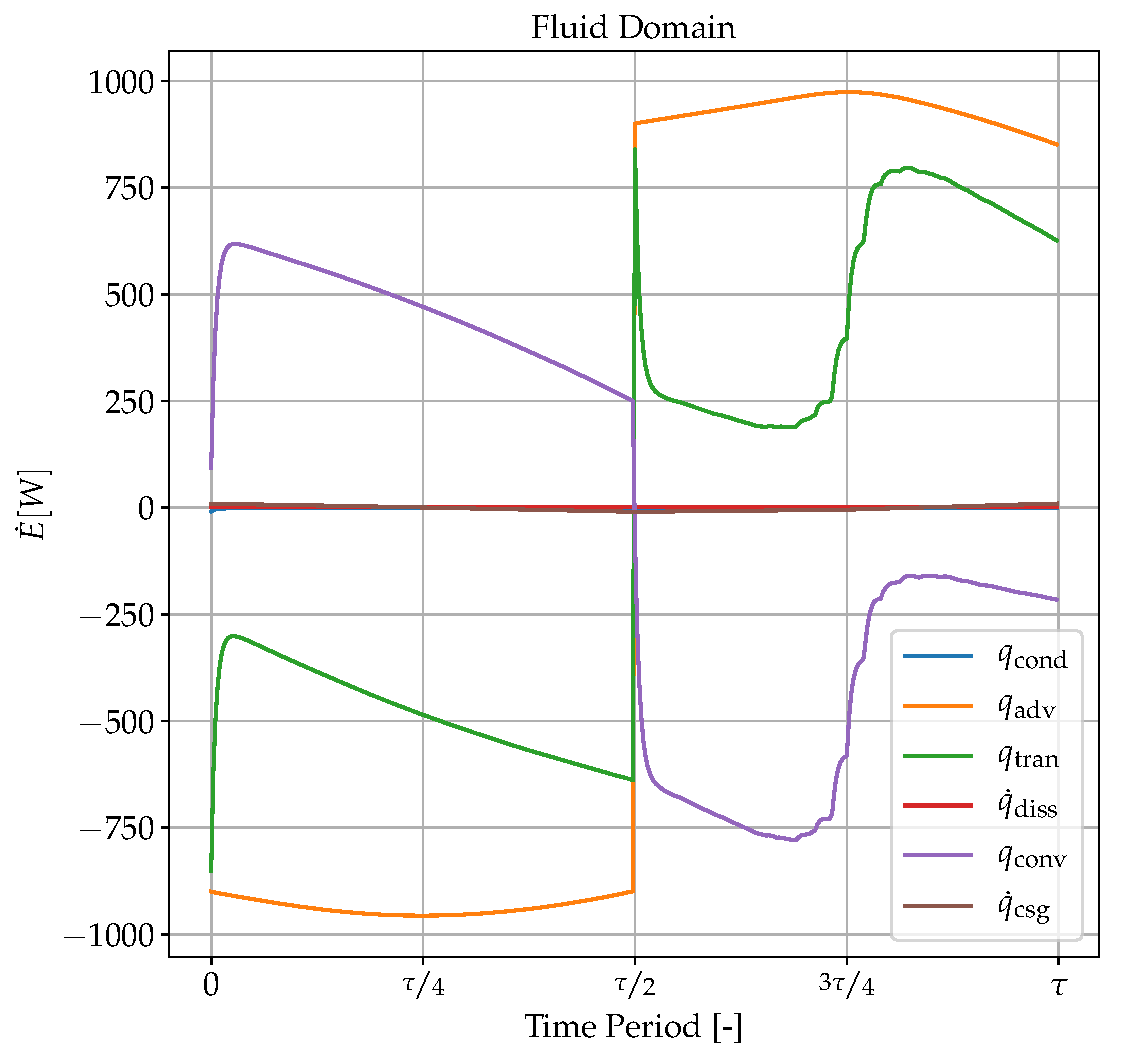
\includegraphics[scale=0.6]{CE_fluid_1_teste.pdf}
  \caption{Energy balance for the fluid domain, using the parameters of AMR 1 given in Table \ref{tab:mesh_cases}.}
  \label{fig:CE_fluid_1}
\end{figure}

\begin{figure}[!ht]
  \centering
  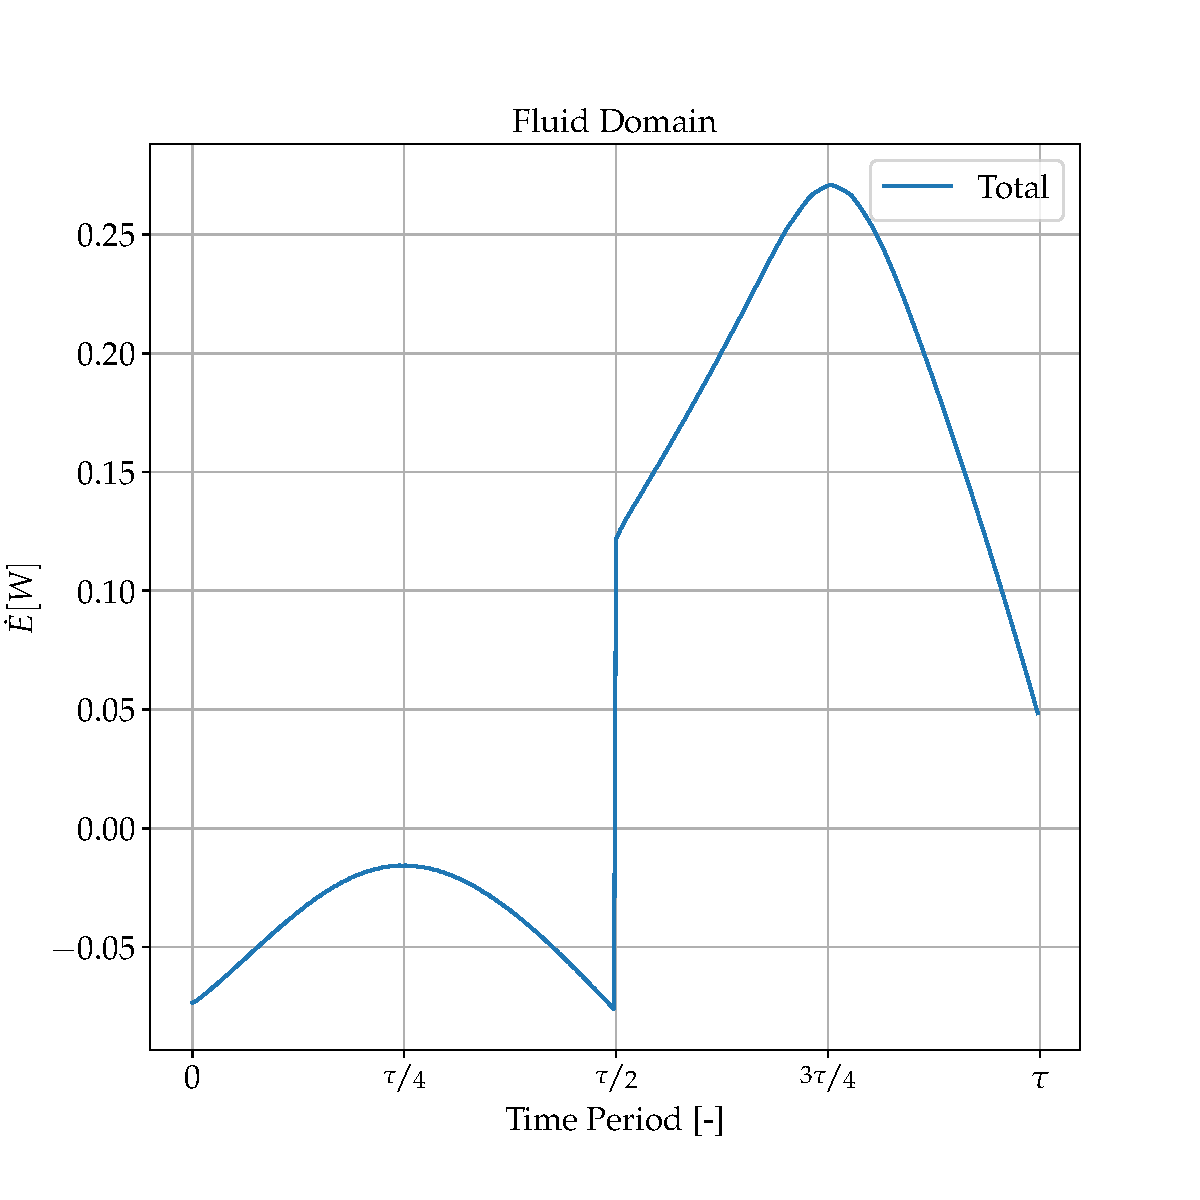
\includegraphics[scale=0.6]{CE_fluid_3.pdf}
  \caption{Sum of the heat fluxes as pointed by Eq.~\eqref{En_bal_f}: (a) Using the criteria defined in Section \ref{subsec:conv-crit} ($\varepsilon_\textrm{cycle}= 10^{-3}$ and $\varepsilon_\textrm{conv} = 10^{-4}$) and; (b) Using the criteria $\varepsilon_\textrm{cycle}= \varepsilon_\textrm{conv} = 10^{-8}$.}
  \label{fig:CE_fluid_2}
\end{figure}

\begin{figure}[!ht]
  \centering
  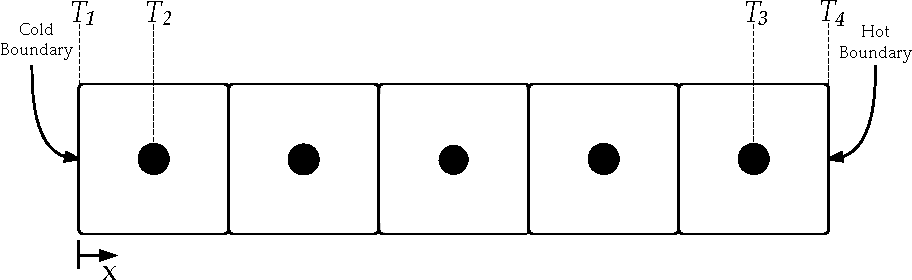
\includegraphics[scale=0.8]{CE_fluid_adv.pdf}
  \caption{Schematic representation of the points where temperature values are known.}
  \label{fig:CE_fluid_adv}
\end{figure}

Fig. \ref{fig:CE_fluid_adv} presents four temperatures $T_1, T_2, T_3, T_4$, and their position in the fluid domain. Due to the prescribed temperature and adiabatic boundary condition, the known temperature in the CB are $T_1$ and $T_3$, and in the HB $T_2$ and $T_4$. But, to calculate correctly the advective term, it would be necessary to know the values of $T_1$ and $T_4$ in the same blow, what is not possible due to the boundary conditions. This error could be minimized with a refined mesh, since $T_2$ and $T_3$ would approximate $T_1$ and $T_4$, or by using a non-linear grid spacing, where the volumes near the extremities should be smaller. Nevertheless the residual energy shown in Fig. \ref{fig:CE_fluid_2} (b) is considered small comparing to the scale. In fact, the temperatures at the boundaries could be obtained by the energy balance in the domain or in the first and last volumes, for a more precisely calculation of $\dot{Q}_\textrm{C}$ and $\dot{Q}_\textrm{H}$, respectively.

\subsection{Casing Domain}


\begin{figure}[!ht]
  \centering
  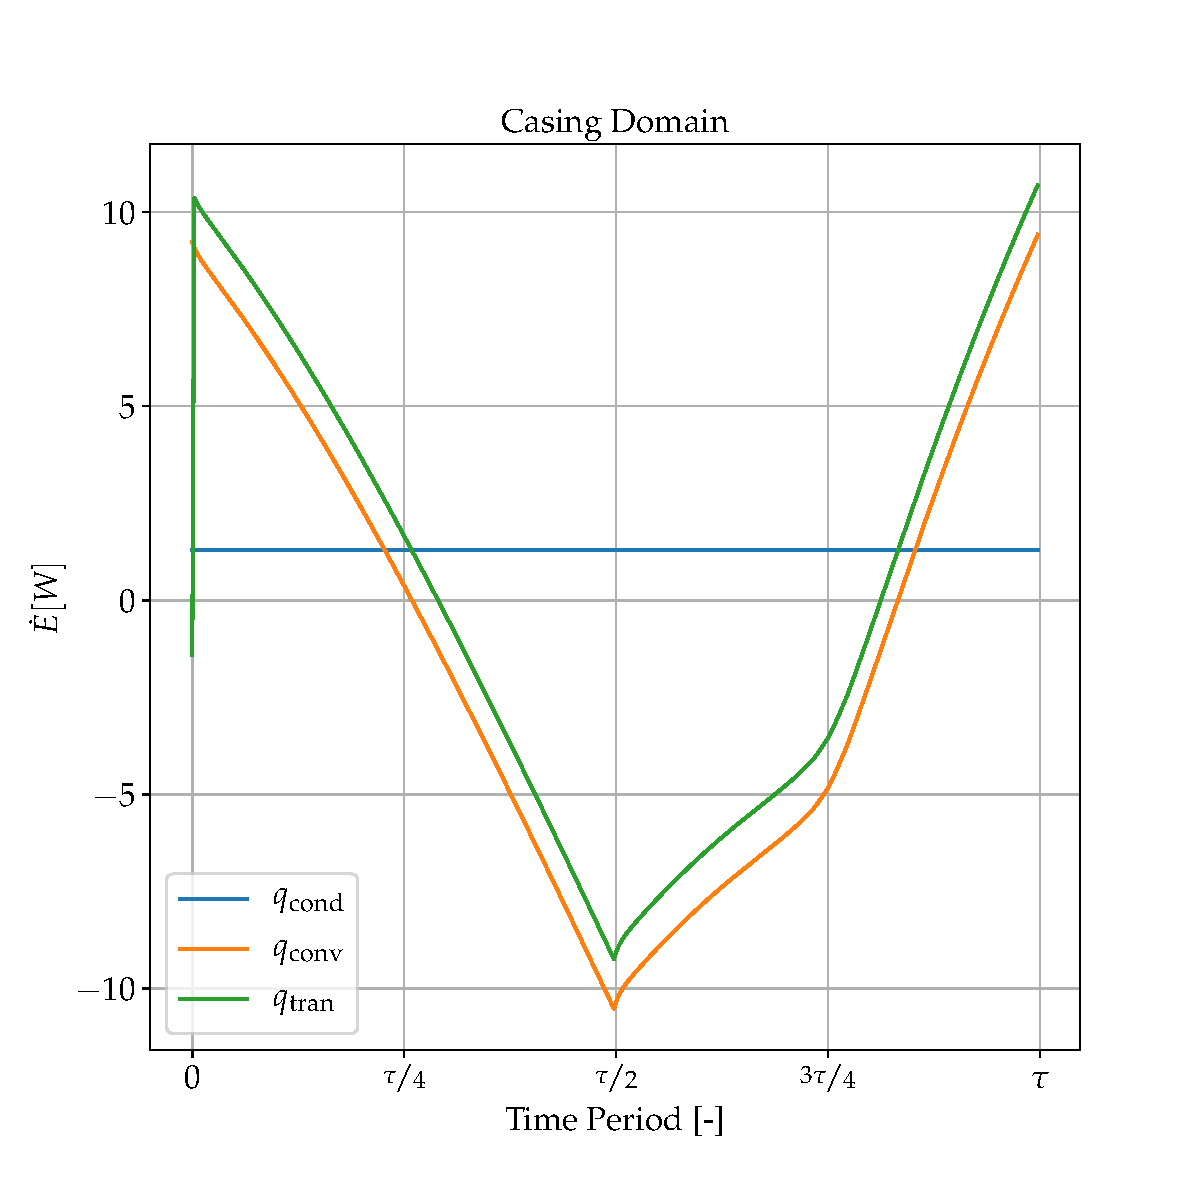
\includegraphics[scale=0.6]{CE_casing_1.pdf}
  \caption{Energy balance for the casing domain, using the parameters of AMR 1 given in Table \ref{tab:mesh_cases}.\textcolor{red}{refazer essa figura}}
  \label{fig:CE_csg_1}
\end{figure}


\begin{figure}[!ht]
  \centering
  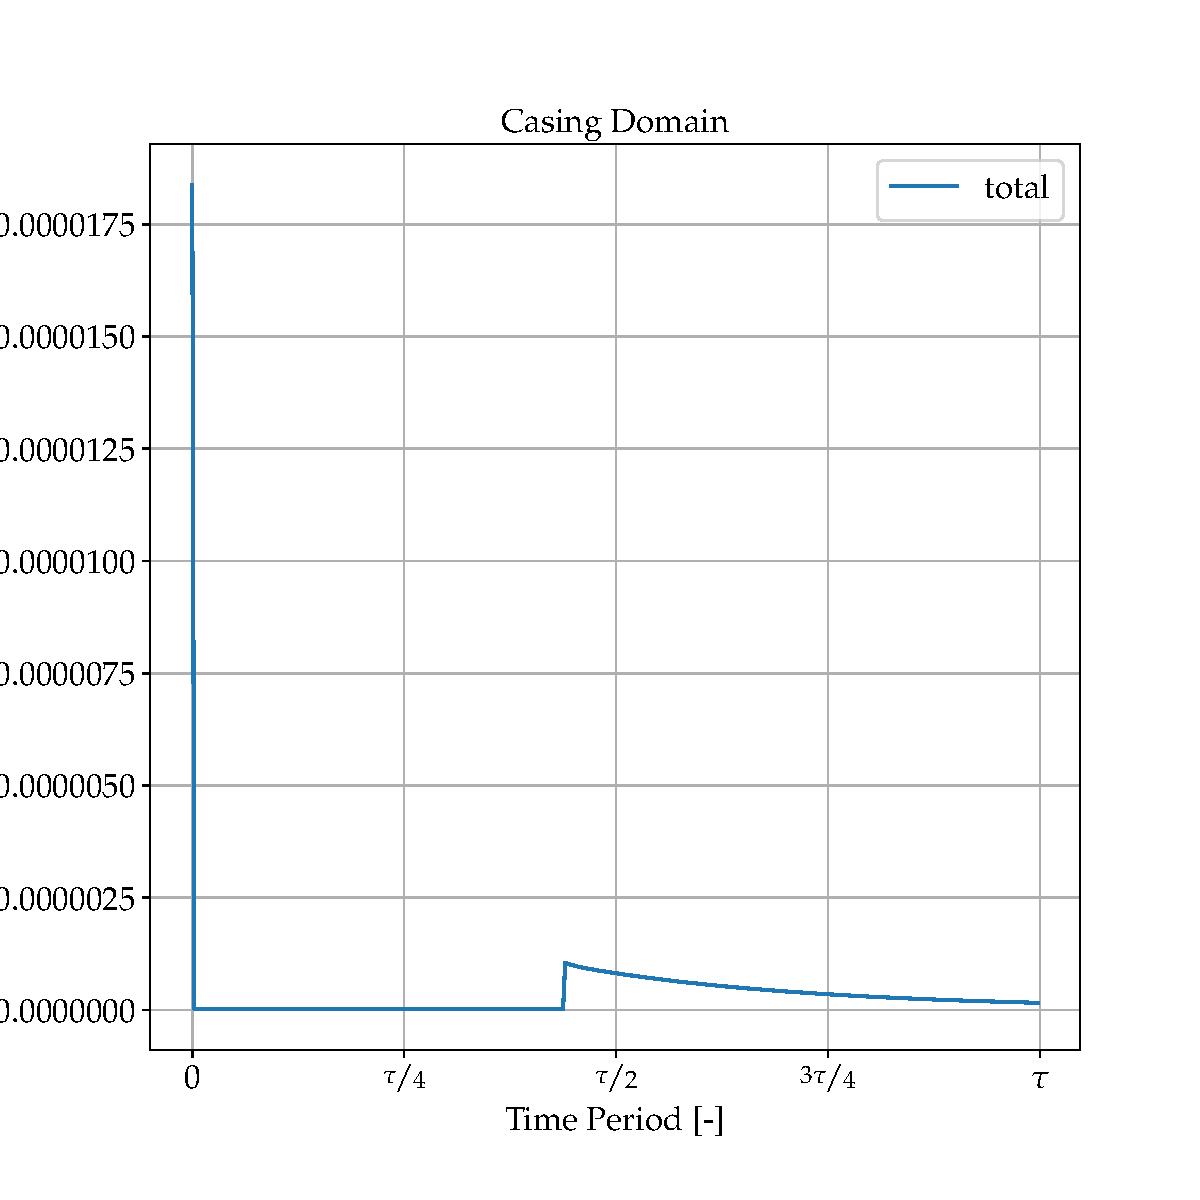
\includegraphics[scale=0.6]{CE_casing_3.pdf}
  \caption{Sum of the heat fluxes as pointed by Eq.~\eqref{En_bal_csg}: (a) Using the criteria defined in Section \ref{subsec:conv-crit} ($\varepsilon_\textrm{cycle}= 10^{-3}$ and $\varepsilon_\textrm{conv} = 10^{-4}$) and; (b) Using the criteria $\varepsilon_\textrm{cycle}= \varepsilon_\textrm{conv} = 10^{-8}$.\textcolor{red}{refazer essa figura}}
  \label{fig:CE_csg_2}
\end{figure}



\section{Results and Discussion}

\subsection{MCE and Losses Validation}

\textcolor{red}{Colocar perfis de temperatura mesmo sem modelo de volume morto?}

Ref. \ref{fig:results_losses} shows the comparison between numerical and experimental results for $\dot{Q}_\textrm{C}$ as a function of $\Delta T_\textrm{span}$ for different values of frequency (0.5 and 1.0Hz) and utilization (0.41, 0.62 and 0.83). The curves are labelled as: (i) "No Losses", which consider only the fluid and solid energy equations and neglecs the demagnetization field; (ii) "Magnetic Losses", which includes the losses due to the demagnetization field; (iii) "Magnetic and Thermal Losses", which also considers the losses due to casing energy interaction and; (iv) "Experimental", which correspond to the experiments carried out by \cite{Trevizoli2015} with the operating conditions as the numerical simulations.

\begin{figure}[htp]
\subfloat{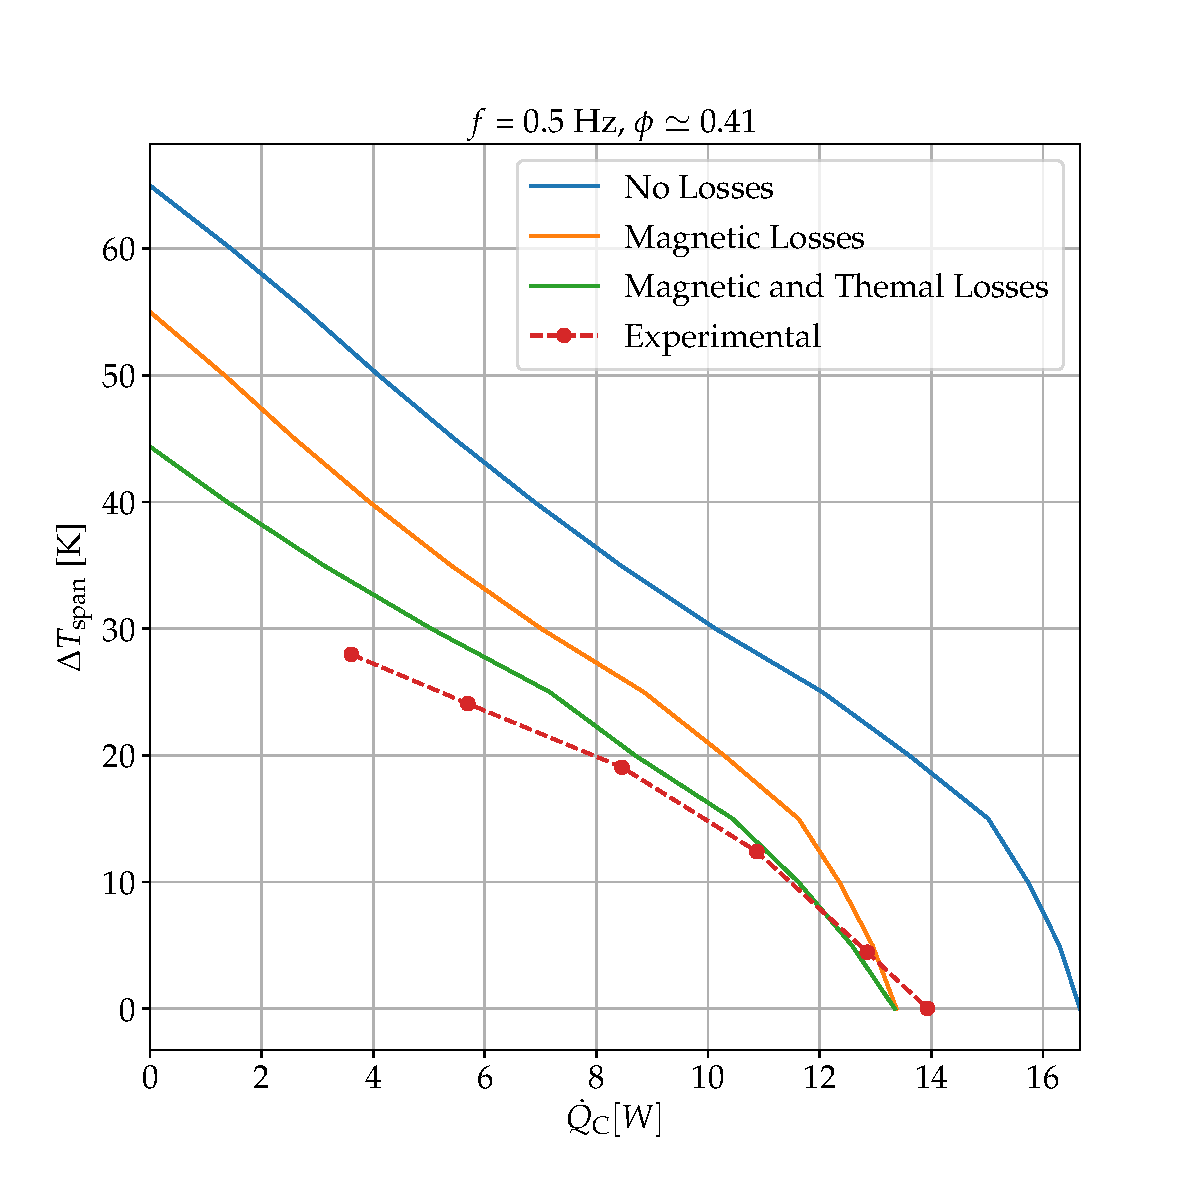
\includegraphics[height=3in]{Losses_result_f_5_phi_41.pdf}}
\subfloat{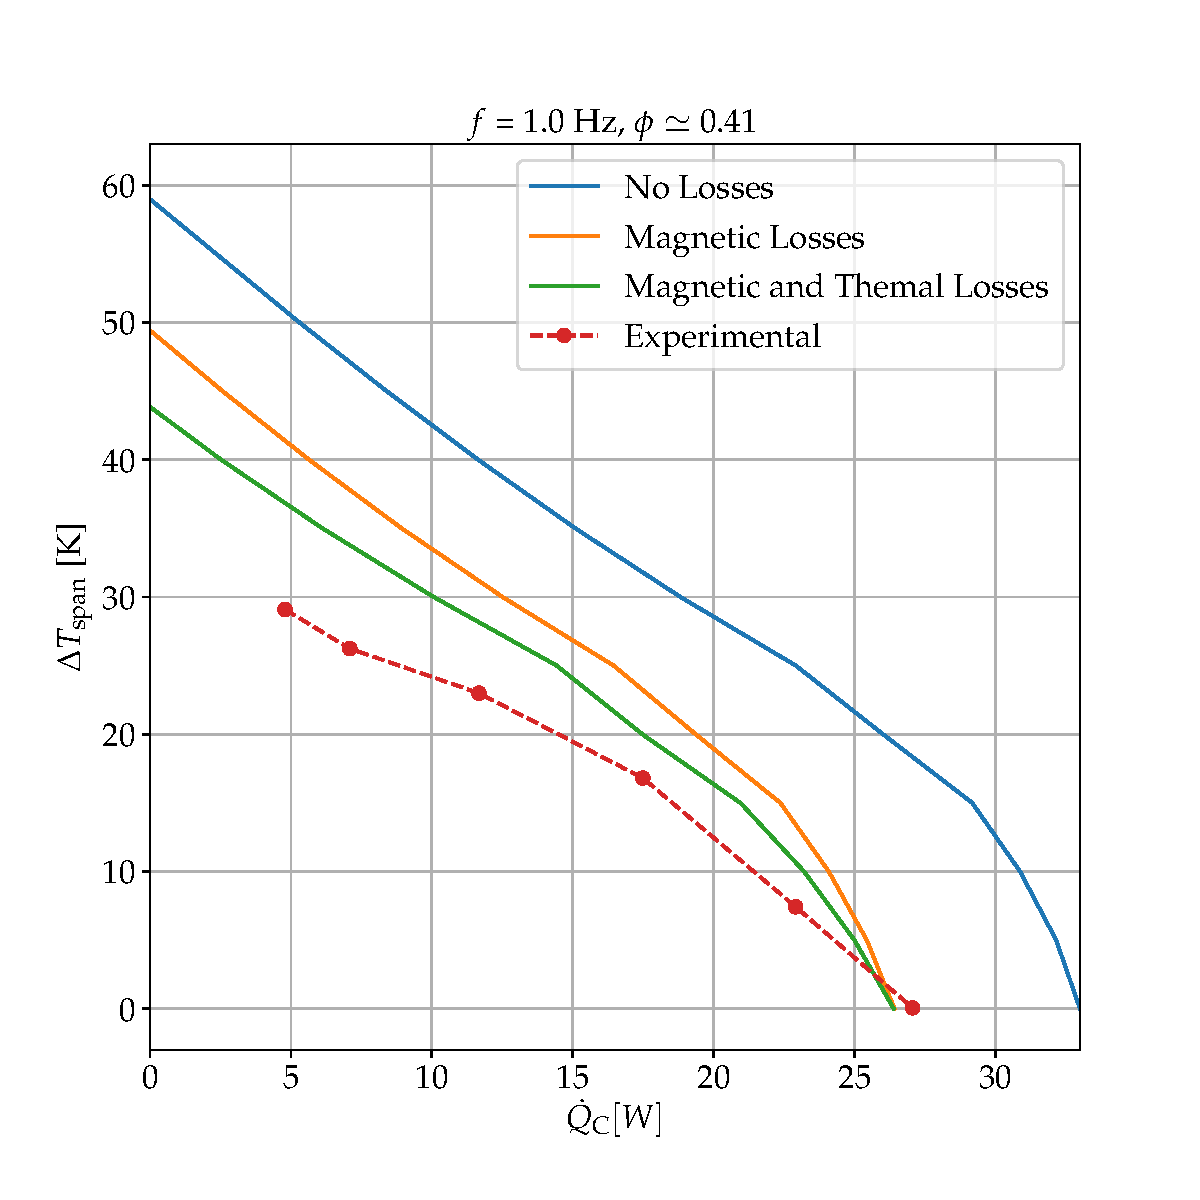
\includegraphics[height=3in]{Losses_result_f_10_phi_41.pdf}}\\
\subfloat{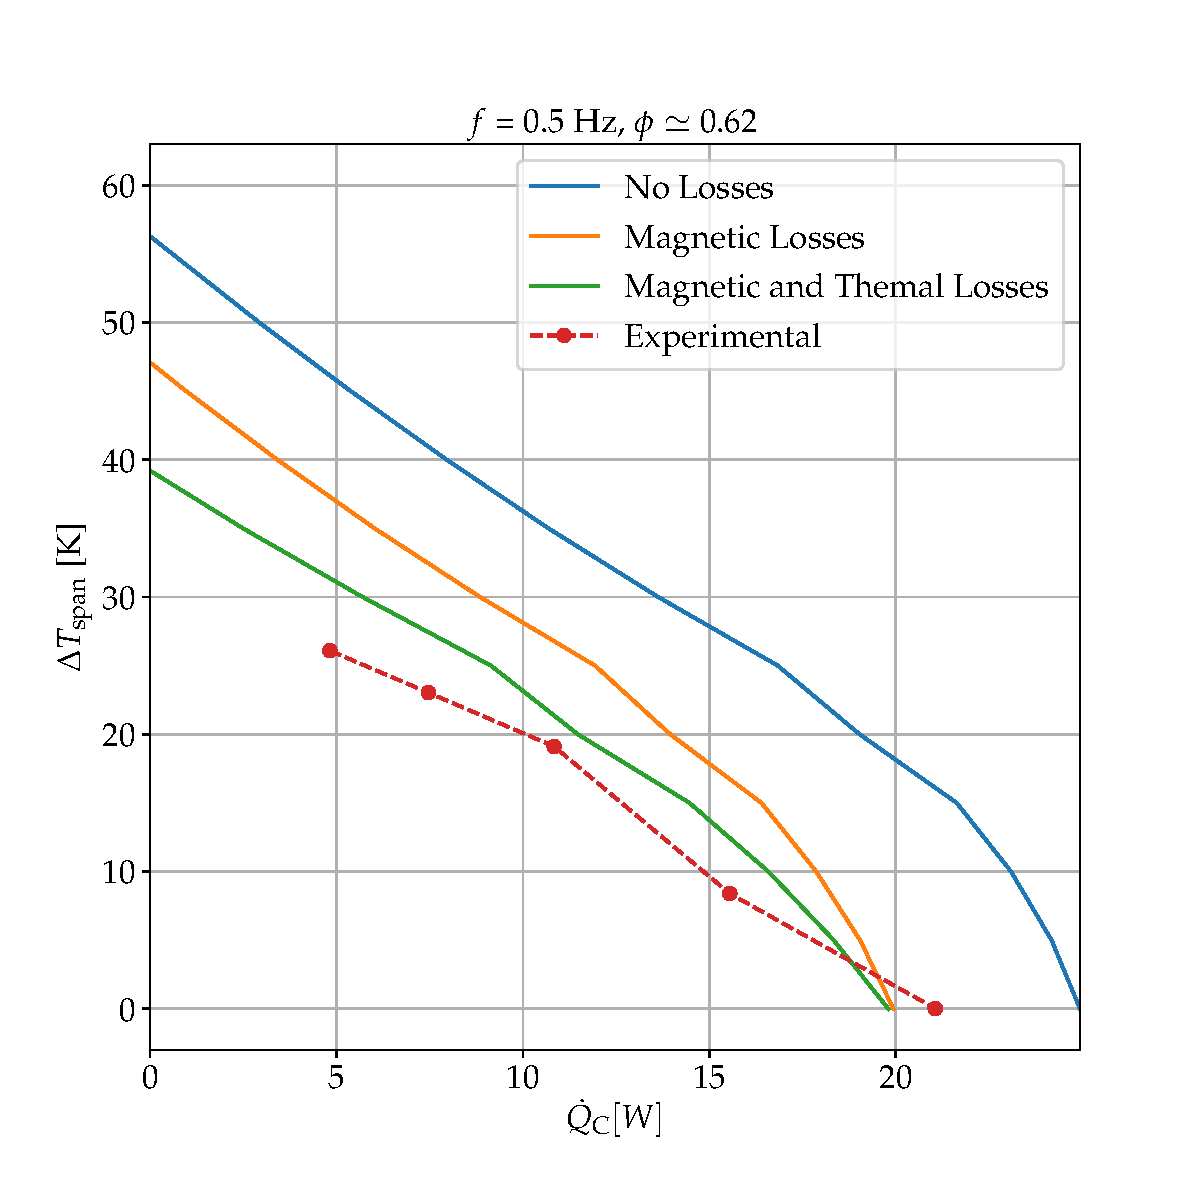
\includegraphics[height=3in]{Losses_result_f_5_phi_62.pdf}}
\subfloat{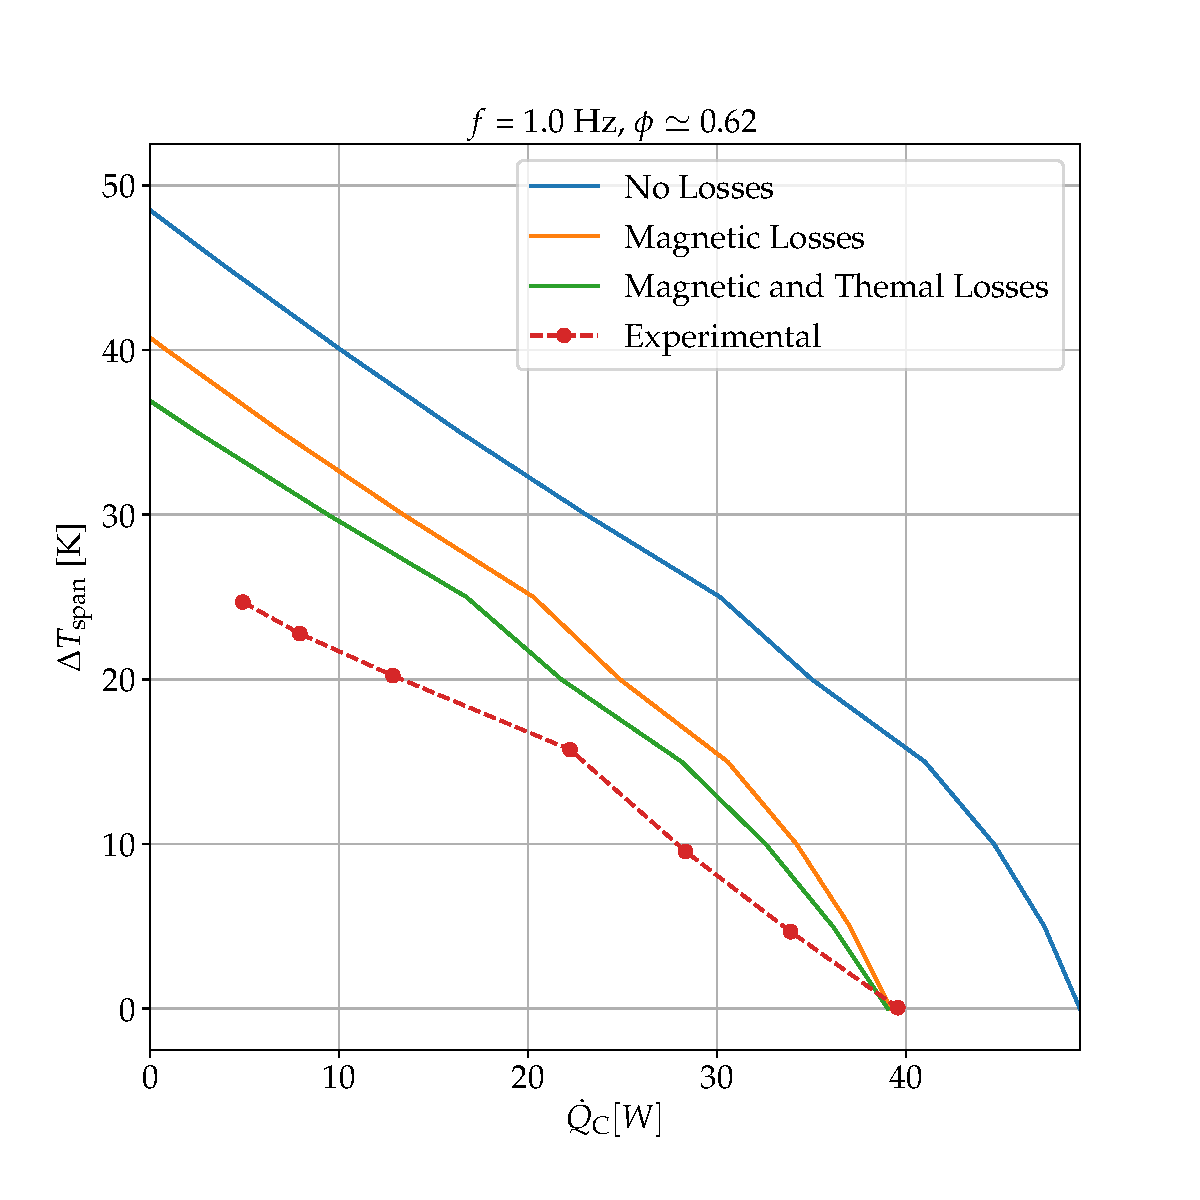
\includegraphics[height=3in]{Losses_result_f_10_phi_62.pdf}}\\
\subfloat{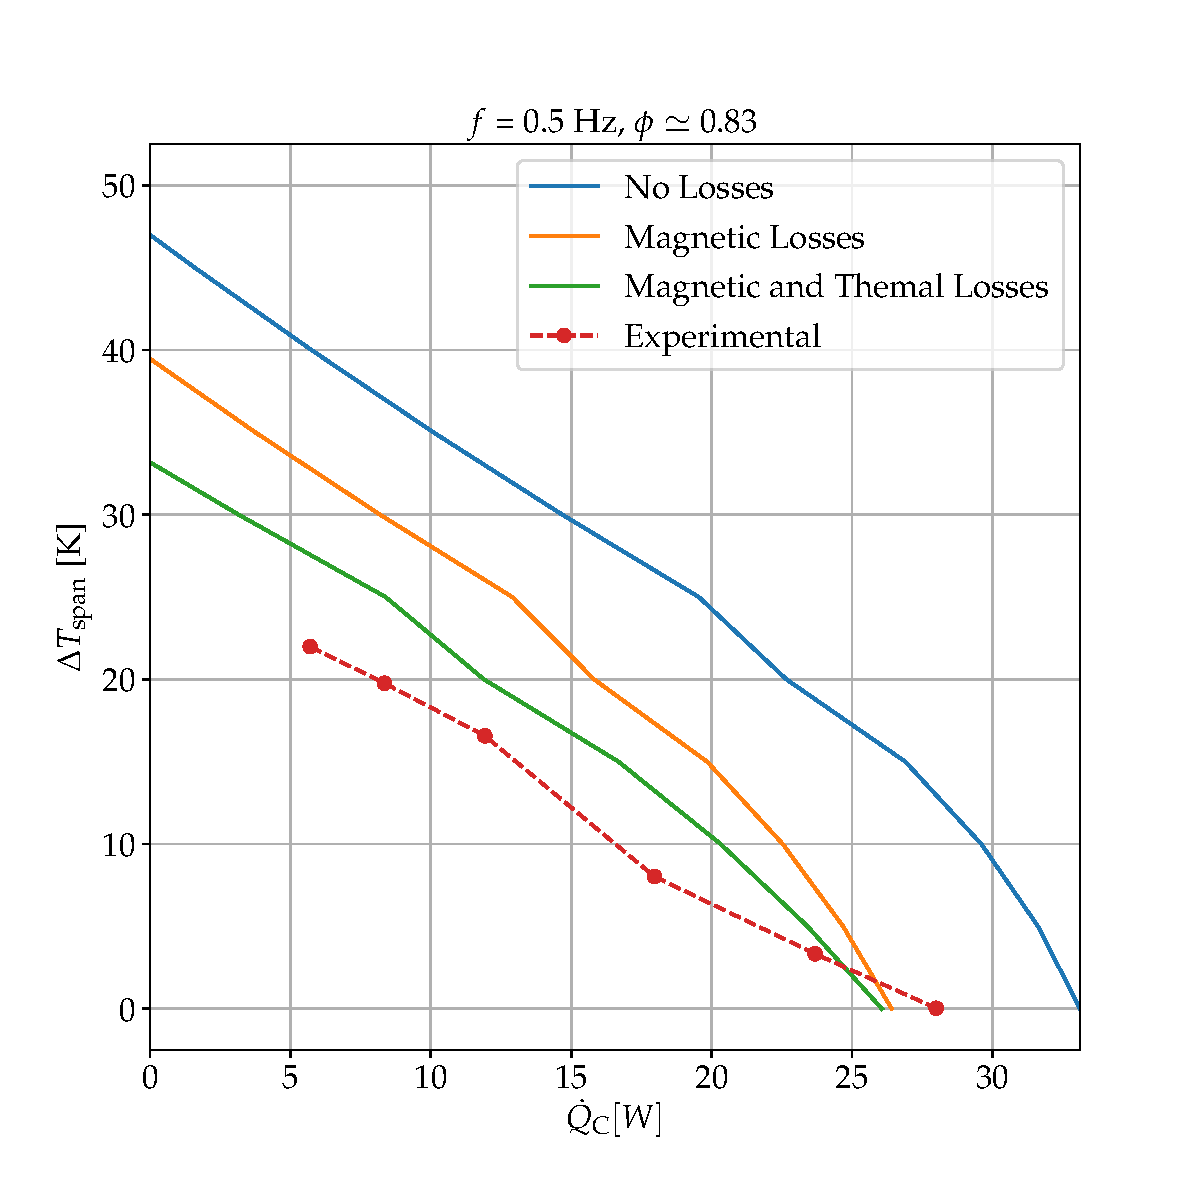
\includegraphics[height=3in]{Losses_result_f_5_phi_83.pdf}}
\subfloat{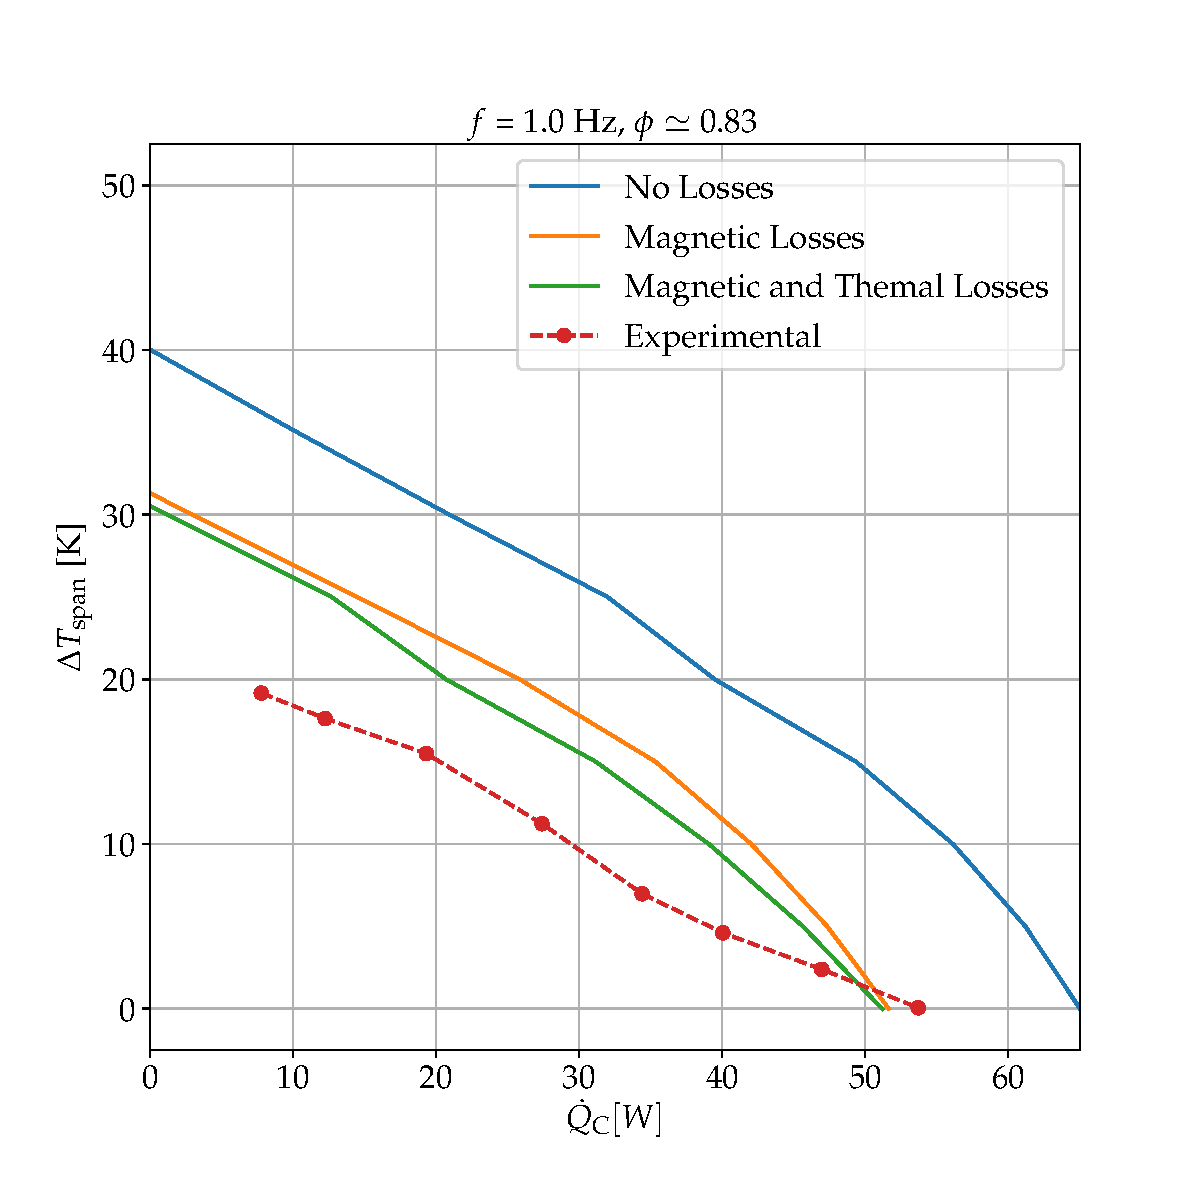
\includegraphics[height=3in]{Losses_result_f_10_phi_83.pdf}}\\

\caption{Comparison between the numerical model and \cite{Trevizoli2015} experimental results considering different types of losses for different frequencies and utilization factors.} 
\label{fig:results_losses}
\end{figure}

A large difference can be seen between the blue and orange lines in Fig. \ref{fig:results_losses}, which represents the losses due to the demagnetization field, pointing out that they are crucial and should be always considered when AMRs are evaluated. In practice, the meaning of the demagnetization field is an internal reduction of the magnetic flux density in the MCM. As the $\Delta T_\textrm{span}$ increases, the thermal losses get more relevant, as the temperature difference between the ambient and the cold end increases. As seen in Fig. \ref{fig:results_losses} the thermal losses are less significant when increasing frequency (as the green and orange lines are closer for higher frequency), since the complete AMR period is shorter and consequently there is less time for thermal interaction between the AMR and the ambient. 

Most of numerical results overestimated the experimental results, expecially at higher $\Delta T_\textrm{span}$. This fact was expected, and may be due to the lack of the void volume \cite{Trevizoli2015,LeiPHD} that was not implemented in the numerical model due time limitations. The void volume is defined as the volume of fluid between each regenerator end and its corresponding heat exchanger that changes direction outside the regenerator, without interacting thermally with it. The void volume fraction, $\upsilon^*$, is defined as the ratio between the total void volume, $\upsilon$, and the fluid volume in the regenerator, $\varepsilon A_\textrm{c,Reg} L$ \cite{Trevizoli2015}:

Fig. \ref{fig:pg255} (a) and (b) show a more complete analysis for $\dot{Q}_\textrm{C}$ as a function of $\phi$ at different $\Delta T_\textrm{span}$ between the numerical results (considering magnetic and thermal losses) and experimental results form \cite{Trevizoli2015} for frequencies of 0.5 and 1 Hz.

\begin{figure}[htp]
\centering
\subfloat[]{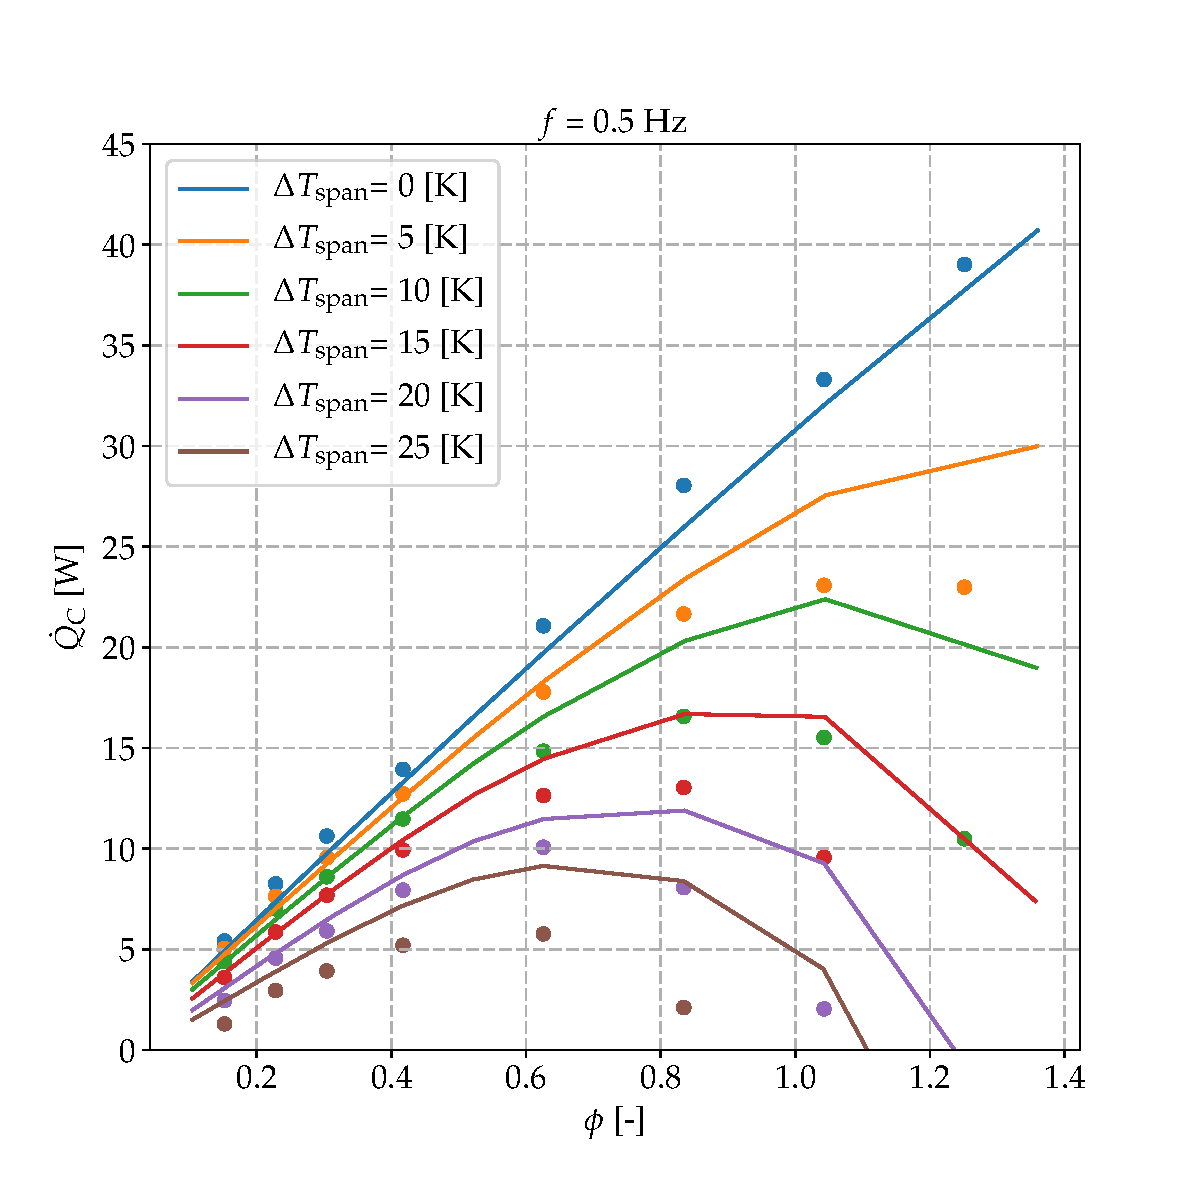
\includegraphics[height=4.5in]{Result_pg255_5.pdf}}\\
\subfloat[]{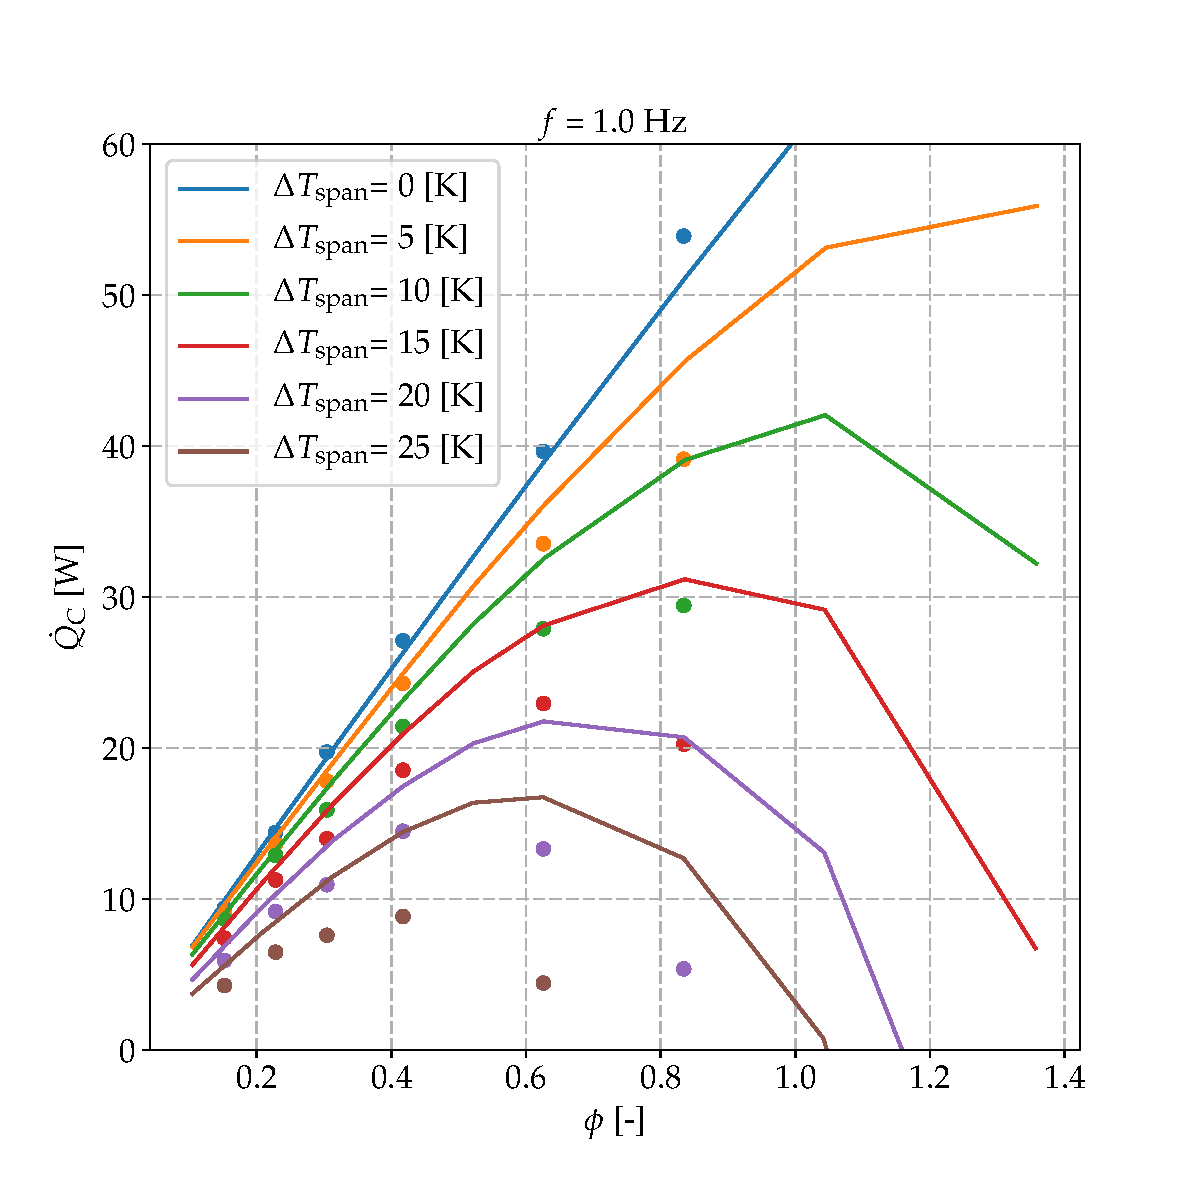
\includegraphics[height=4.5in]{Result_pg255_10.pdf}}\\
\caption{Comparison between the numerical results (full lines) and \cite{Trevizoli2015} experimental data (dots) of the cooling power as function of the utilization factor for different temperature spans: (a) $f$ = 0.5 Hz; (b) $f$ = 1 Hz.}
\label{fig:pg255}
\end{figure}

At zero temperature span, a slightly underestimation of the numerical cooling power is noticed for all utilization factors. For the other temperature spans, in general it is noticed an increase in the $\dot{Q}_\textrm{C}$ overestimation with increasing utilization factors. Also, an increase in the $\dot{Q}_\textrm{C}$ overestimation occurs with increasing $\Delta T_\textrm{span}$. For instance, at $f$ = 0.5 Hz and $\phi \simeq$ 0.4, as the $\Delta T_\textrm{span}$ is increased, the deviation between the numerical and experimental results grows.

Overestimated conditions reinforce the previously suggested $Nu_\textrm{csg}$ correlation errors, since the heat losses to the surrounding are higher for larger $\Delta T_\textrm{span}$, due to larger temperature differences between the cold end and the ambient, and for higher utilization factors, due to larger convection coefficients relative to larger mass flow rates. It is important to point out that the void volumes losses are not taken into account here. \cite{Trevizoli2015} also reported a numerical underestimation of $\dot{Q}_\textrm{C}$ for the $\Delta T_\textrm{span}$ of 0 K, and with the void volume model this difference was reduced.

For lower utilization factors, the numerical results are in good agreement with the experimental data for both frequencies. While for higher utilization factors, the numerical results reproduced the experimental trends quite well, exhibiting a maximum deviation of about 10 W.

\subsection{Blow Fraction Validation}

\textcolor{red}{Se colocar essa seção precisa explicar em algum lugar o conceito de blow fraction}


\cite{Nakashima2017} validated the numerical model developed by \cite{Trevizoli2015}, evaluating the influence of different blow fractions in the performance of AMRs. Also, \cite{Nakashima2017} modified the experimental apparatus developed by \cite{Trevizoli2015} adapting the AMR with a gear pump and two rotary valves, to change the flow profile from sinusoidal to a ramp profile and enable $F_\textrm{b}$ variation. However, for the following numerical results, an instantaneous flow profile was considered to simplify the analysis. As the experimental ramp period was short, the simplification of the flow profile is acceptable. A schematic representation of blow fraction was presented in Fig. \ref{fig:Fb}. All the other parameters are the same as those summarized in Table \ref{tab:par_paulo}. The comparison between the numerical and experimental results of $\dot{Q}_\textrm{C}$ as a function of the utilization factor is shown in Fig. \ref{fig:Alan}.

\begin{figure}[htp]
\centering
\subfloat[]{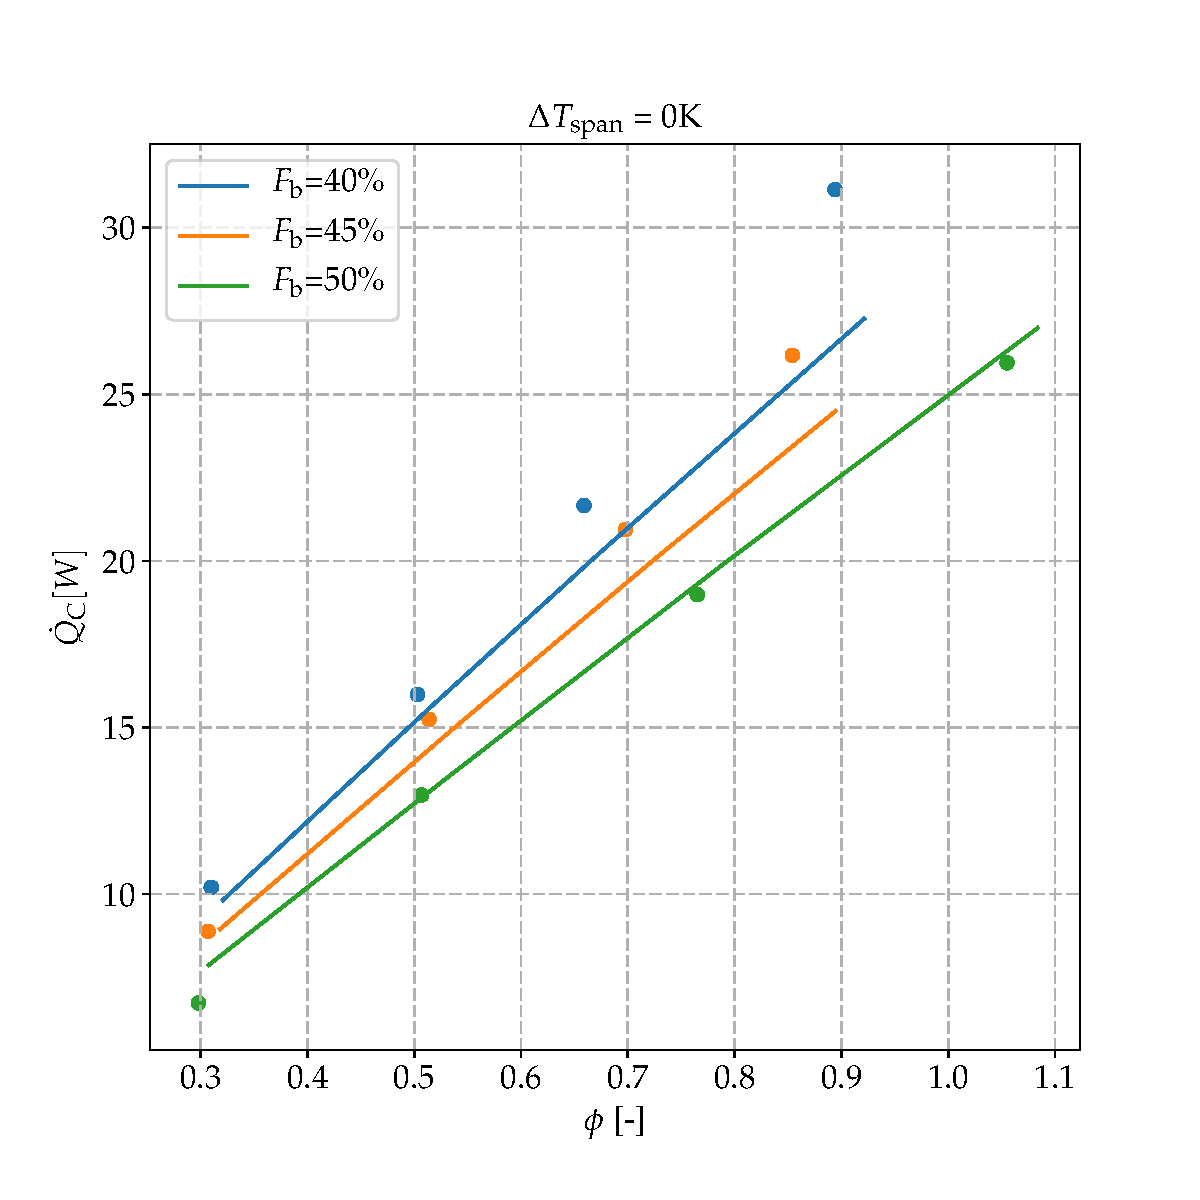
\includegraphics[height=4.5in]{Alan_span_0.pdf}}\\
\subfloat[]{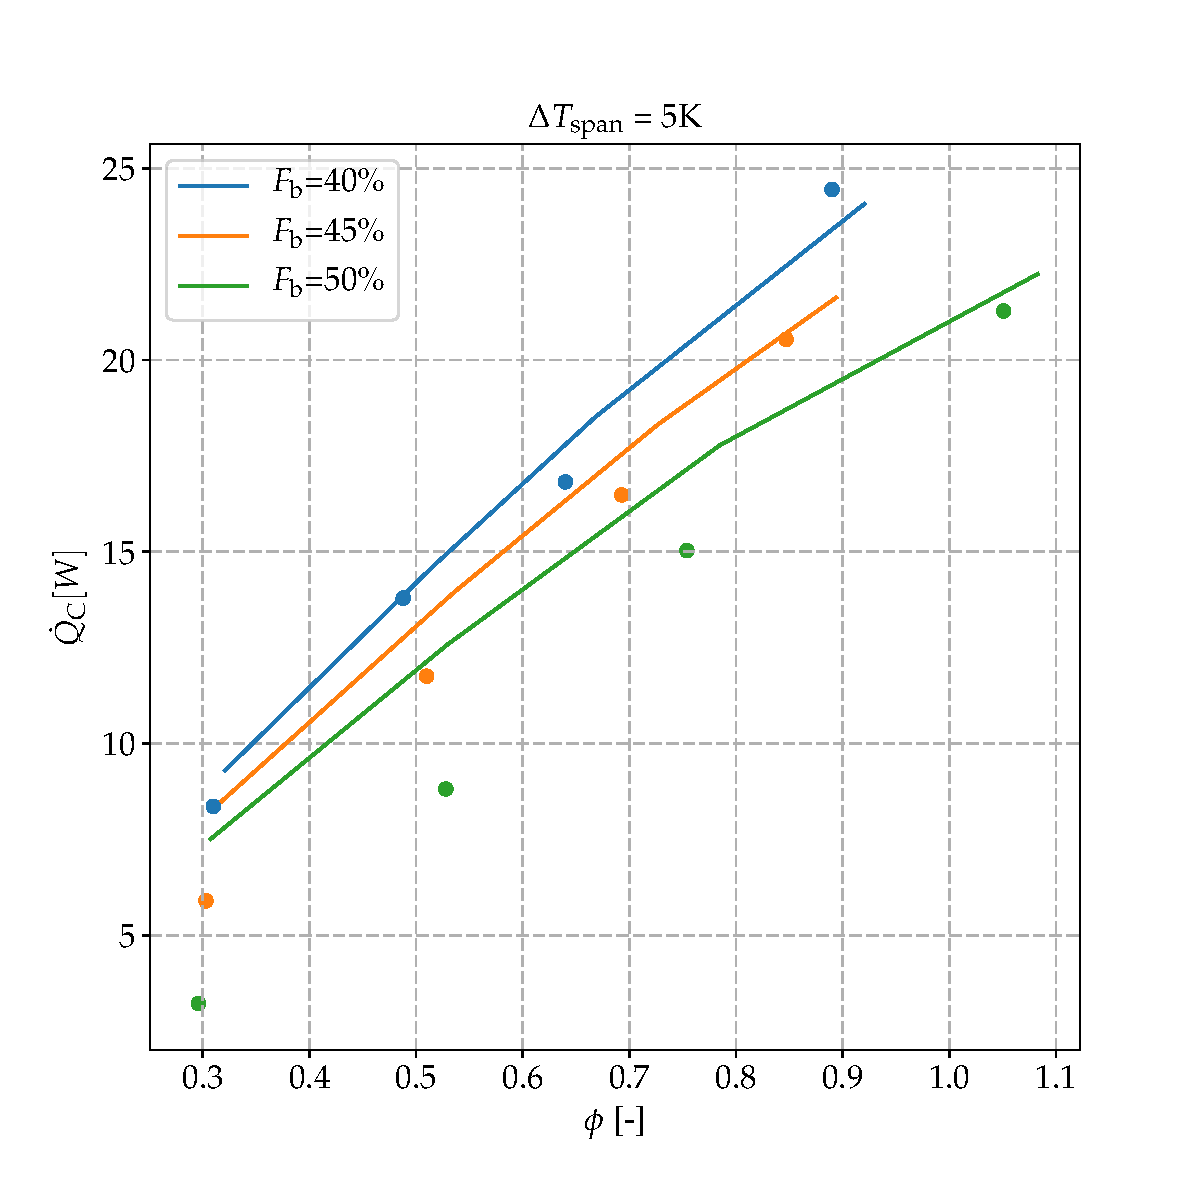
\includegraphics[height=4.5in]{Alan_span_5.pdf}}\\
\caption{Comparison between the numerical results (full lines) and the experimental data obtained by \cite{Nakashima2017} (dots) at: (a) $\Delta T_\textrm{span}$ = 0 K; (b) $\Delta T_\textrm{span}$ = 5 K.}
\label{fig:Alan}
\end{figure}

The blow fraction can be employed to increase the AMR performance by better exploration of the magnetic flux density variation \cite{Teyber2016,Nakashima2017}. As can be noticed in Fig. \ref{fig:Alan}, and similar to the experimental results, $\dot{Q}_\textrm{C}$ calculated from the numerical results always increase when decreasing the blow fraction, at the different utilization factors and temperature spans simulated in this work. 

In general, the numerical results are in good agreement with the experimental data. For $\Delta T_\textrm{span}$ = 0 K, except for $\phi \simeq$  0.9 and $F_\textrm{b}$ = 40\%, all the experimental points were well predicted by the model. For $\Delta T_\textrm{span}$ = 5 K, the numerical model overpredicted $\dot{Q}_\textrm{C}$ in some points, especially for $F_\textrm{b}$ = 50\% and lower utilization factors. An important issue to point out, is that the uncertainty of the experimental results obtained by \cite{Nakashima2017} is larger than those performed by \cite{Trevizoli2015}. Even though the same apparatus was employed, the adaptation of the hydraulic circuit carried out by \cite{Nakashima2017}, increased the mass unbalance \cite{EriksenPHD,Nakashima2017}, which was not included in the numerical simulations shown in Fig. \ref{fig:Alan}.


\subsection{Multilayer Validation}

\textcolor{red}{acho que nao da pra colocar essa secao pq sao os mesmo resultados do paper do henrique}



\subsection{First Order Materials Results}

\textcolor{red}{nao tem comparacao experimental, nao sei se adianta colocar essa seção}

\section{Conclusions}


\section*{References}

\bibliographystyle{elsarticle-num}


\bibliography{References_gusttav}

\end{document}